%% Copernicus Publications Manuscript Preparation Template for LaTeX Submissions
\documentclass[gmd, manuscript]{copernicus} %final manuscript

\begin{document}
\title{Globally-gridded mean climatological crop model emulators for yield and irragation water demand}

\Author[1,2]{James}{Franke}
\Author[3]{Christoph}{M\"{u}ller}
\Author[2,4]{Joshua}{Elliott}
\Author[5]{Alexander}{Ruane}
\Author[6]{Abigail}{Snyder}
\Author[3,2,4,5]{Jonas}{J\"{a}germeyr}
\Author[7,8]{Juraj}{Balkovic}
\Author[9,10]{Philippe}{Ciais}
\Author[11]{Marie}{Dury}
\Author[12]{Pete}{Falloon}
\Author[7]{Christian}{Folberth}
\Author[11]{Louis}{Fran{\c{c}}ois}
\Author[13]{Tobias}{Hank}
\Author[14,23]{Munir}{Hoffmann}
\Author[15,16]{R.\ Cesar}{Izaurralde}
\Author[11]{Ingrid}{Jacquemin}
\Author[15]{Curtis}{Jones}
\Author[7]{Nikolay}{Khabarov}
\Author[14]{Marian}{Koch}
\Author[2,17]{Michelle}{Li}
\Author[9,18]{Wenfeng}{Liu}
\Author[19]{Stefan}{Olin}
\Author[5,20]{Meridel}{Phillips}
\Author[21,22]{Thomas A.\ M.}{Pugh}
\Author[15]{Ashwan}{Reddy}
\Author[9,10]{Xuhui}{Wang}
\Author[12]{Karina}{Williams}
\Author[13]{Florian}{Zabel}
\Author[1,2]{Elisabeth}{Moyer}
%%%%%%%%%%%%%%%%%%%%%%%%%%%%%%
\affil[1]{Department of the Geophysical Sciences, University of Chicago, Chicago, IL, USA}
\affil[2]{Center for Robust Decision-making on Climate and Energy Policy (RDCEP), University of Chicago, Chicago, IL, USA}
\affil[3]{Potsdam Institute for Climate Impact Research, Member of the Leibniz Association, Potsdam, Germany}
\affil[3]{Department of Computer Science, University of Chicago, Chicago, IL, USA}
\affil[5]{NASA Goddard Institute for Space Studies, New York, NY, United States}
\affil[6]{Joint Global Change Research Institute, Pacific Northwest National Laboratory, College Park, MD, USA}
\affil[7]{Ecosystem Services and Management Program, International Institute for Applied Systems Analysis, Laxenburg, Austria}
\affil[8]{Department of Soil Science, Faculty of Natural Sciences, Comenius University in Bratislava, Bratislava, Slovak Republic}
\affil[9]{Laboratoire des Sciences du Climat et de l'Environnement, CEA-CNRS-UVSQ, 91191 Gif-sur-Yvette, France}
\affil[10]{Sino-French Institute of Earth System Sciences, College of Urban and Env. Sciences, Peking University, Beijing, China}
\affil[11]{Unit{\'{e}} de Mod{\'{e}}lisation du Climat et des Cycles Biog\'eochimiques, UR SPHERES, Institut d'Astrophysique et de G\'eophysique, University of Li\`ege, Belgium}
\affil[12]{Met Office Hadley Centre, Exeter, United Kingdom}
\affil[13]{Department of Geography, Ludwig-Maximilians-Universit\"{a}t, Munich, Germany}
\affil[14]{Georg-August-University G\"{o}ttingen, Tropical Plant Production and Agricultural Systems Modelling, G\"{o}ttingen, Germany}
\affil[15]{Department of Geographical Sciences, University of Maryland, College Park, MD, USA}
\affil[16]{Texas Agrilife Research and Extension, Texas A\&M University, Temple, TX, USA}
\affil[17]{Department of Statistics, University of Chicago, Chicago, IL, USA}
\affil[18]{EAWAG, Swiss Federal Institute of Aquatic Science and Technology, D\"{u}bendorf, Switzerland}
\affil[19]{Department of Physical Geography and Ecosystem Science, Lund University, Lund, Sweden}
\affil[20]{Earth Institute Center for Climate Systems Research, Columbia University, New York, NY, USA}
\affil[21]{School of Geography, Earth and Environmental Sciences, University of Birmingham, Birmingham, UK.}
\affil[22]{Birmingham Institute of Forest Research, University of Birmingham, Birmingham, UK.}
\affil[23]{Leibniz Centre for Agricultural Landscape Research (ZALF), D-15374 Müncheberg, Germany}

%%%%%%%%%%%%%%%%%%%%%%%%%%%%%%
\runningtitle{The GGCMI Phase II experiment: simulating and emulating global crop yield}
\runningauthor{Franke et al.}
\correspondence{James Franke (jfranke@uchicago.edu)}
%%%%%%%%%%%%%%%%%%%%%%%%%%%%%%
%% These dates will be inserted by Copernicus Publications during the typesetting process.
\received{}
\pubdiscuss{} %% only important for two-stage journals
\revised{}
\accepted{}
\published{}
%%%%%%%%%%%%%%%%%%%%%%%%%%%%%%
\firstpage{1}
\maketitle
%%%%%%%%%%%%%%%%%%%%%%%%%%%%%%
\begin{abstract}
For emulating these responses, the GGCMI Phase II systematic parameter sweep protocol allows disentangling the climate-driven mean response from year-over-year variations; we show that the two responses have very different relationships to standard climate metrics such as mean growing season temperature. 
The climatological mean yield response can be readily represented with a simple polynomial in almost all locations where crops are currently grown, permitting a tool that captures model responses in a lightweight, computationally tractable form. 
Crop model emulation should therefore facilitate both model comparison and integrated assessment of climate impacts.
\end{abstract}

%\copyrightstatement{TEXT}

\introduction
\label{S:1}
Efforts to project climate change impacts often combine models from different disciplines under a single economic framework to calulcate a total cost of climate change or total cost of carbon often called an Integrated Assessment Model (IAM). 
The numerical models implemented by different disciplines studying climate change and its associated impacts cannot be directly integrated into IAMs because of their simulation framework or computational cost. 
Process-based crop simulation models provide many advantages for projecting the impacts of climate change on agriculture but are difficult to directly integrate into larger economic assessments. 
Statistical crop models on the other hand, often lack important features of process-based models including future atmospheric CO$_2$ fertilization and potential changes in agricultural management, but sometimes take analytical forms that can be brought directly into an IAM.

Interest has been rising in statistical emulation, which allows combining advantageous features of both statistical and process-based models. 
The approach involves constructing a statistical representation or ``surrogate model'' of complicated numerical simulations by using simulation output as the training data for a statistical model \citep[e.g.][]{OHAGAN2006, OHAGAN2010}. 
Emulation is particularly useful in cases where simulations are complex and output data volumes are large,  and  has been used in a variety of fields, including hydrology \citep[e.g.][]{Razavi2012}, engineering \citep[e.g.][]{STORLIE2009}, environmental sciences \citep[e.g.][]{RATTO2012}, and climate \citep[e.g.][]{Castruccio14, Holden2014}. 
For agricultural impacts studies, emulation of process-based models allows capturing key relationships between input variables in a lightweight, flexible form that is compatible with economic studies. 

In the past decade, multiple studies have developed emulators of process-based crop simulations. 
Early studies proposing or describing potential crop yield emulators include \citet{Howden2005, raisen2006, Lobell2010}, and \citet{Ferrise2011}, who used a machine learning approach to predict Mediterranean wheat yields. 
Studies developing single-model emulators include  \citet{Holzkamper2012} for the CropSyst model, \citet{RUANE2013a} for the CERES wheat model, and \citet{Oyebamiji15} for the LPJmL model (for multiple crops, using multiple scenarios as a training set). 
More recently, emulators have begun to be used in the context of multi-model intercomparisons, with \citet{BLANC2015, BLANC2017, Ostberg2018} and \citet{Mistry2017} using them to analyze the five crop models of the Inter-Sectoral Impacts Model Intercomparison Project (ISIMIP) \citep{Warszawski3228}, which simulated yields for maize, soy, wheat, and rice. 
Choices differ: \citet{BLANC2015} and \citet{BLANC2017} base their emulation on historical simulations and three climate scenarios for one Representative Concentration Pathway (RPC8.5), which represents a high level of global warming; and use local weather variables and yields in their regression across soil regions; \citet{Ostberg2018} use global mean temperature change (and CO$_2$) as regressors then pattern-scale to emulate local yields; while \citet{Mistry2017} compare emulated and observed historical yields, using local weather data and a historical crop simulation. 
These efforts do share important common features: all emulate annual crop yields across the entire scenario or scenarios, and when future scenarios are considered, they are non-stationary, i.e.\ their input climate parameters evolve over the course of the simulations.

An alternative approach is to construct a training set of multiple stationary scenarios in which parameters are systematically varied. 
Such a ``parameter sweep'' offers several advantages for emulation over scenarios in which climate evolves over time. 
First, it allows separating the effects of different variables that impact yields but that are highly correlated in realistic future scenarios (e.g.\ CO$_2$ and temperature). 
Second, it allows making a distinction between year-over-year yield variations and climatological changes, which may involve different responses to the particular climate regressors used \citep[e.g.][]{Ruane2016}. 
For example, if year-over-year yield variations are driven predominantly by variations in the distribution of temperatures throughout the growing period, and long-term climate changes are driven predominantly by shifts in means, then regressing on the mean growing period temperature will produce different yield responses at annual vs.\ climatological timescales. 
Disadvantages of this approach include neglecting changes in seasonality and some implausible combinations of input settings (e.g. colder temperature and high CO$_2$). 

Systematic parameter sweeps have begun to be used in crop model evaluation and emulation, with early efforts in 2014 and 2015 \citep{ruane2014, Markowski2015, Pirttioja2015}, and several recent studies in 2018 \citep{FRONZEK20182, Snyder2018, RUIZRAMOS2018}. 
All three 2018 studies sample multiple perturbations to temperature and precipitation (with \citet{Snyder2018} and \citet{RUIZRAMOS2018} adding CO$_2$ as well), in 132, 99 and 220 different combinations, respectively, and take advantage of the structured training set to construct emulators (``response surfaces'') of climatological mean yields, omitting year-over-year variations. 
All studies focus on a limited number of sites; \citet{FRONZEK20182} and \citet{RUIZRAMOS2018} simulate only wheat (over many models) and \citet{Snyder2018} analyzes four crops (maize, wheat, rice, soy) for agricultural impacts experiments with the GCAM \citep{calvin2019} model.

In this paper we describe a crop model emulator developed from a new simulation output dataset parameter sweep as part of the Global Gridded Crop Model Intercomparison (GGCMI) Phase II experiment under the Agricultural Model Intercomparison and Improvement Project (AgMIP) \citep{ROSENZWEIG2013, Rosenzweig2014}. 
In this paper we introduce a spatially explicit emulator for the mean-climatological time scale that allows for representing process-based crop model responses in economic assessment models and other applications.

%%%%%%%%%%%%%%%%%%%%%%%%%%%%%%%%%%%%%%%%%%%%%%%%%%%%%%%%%%%%%%%
%%%%%%%%%%%%%%%%%%%%%%%%%%%%%%%%%%%%%%%%%%%%%%%%%%%%%%%%%%%%%%%
%%%%%%%%%%%%%%%%%%%%%%%%%%%%%%%%%%%%%%%%%%%%%%%%%%%%%%%%%%%%%%%
\section{Methods}
\label{S:2}

\begin{figure}[ht]
\centering
   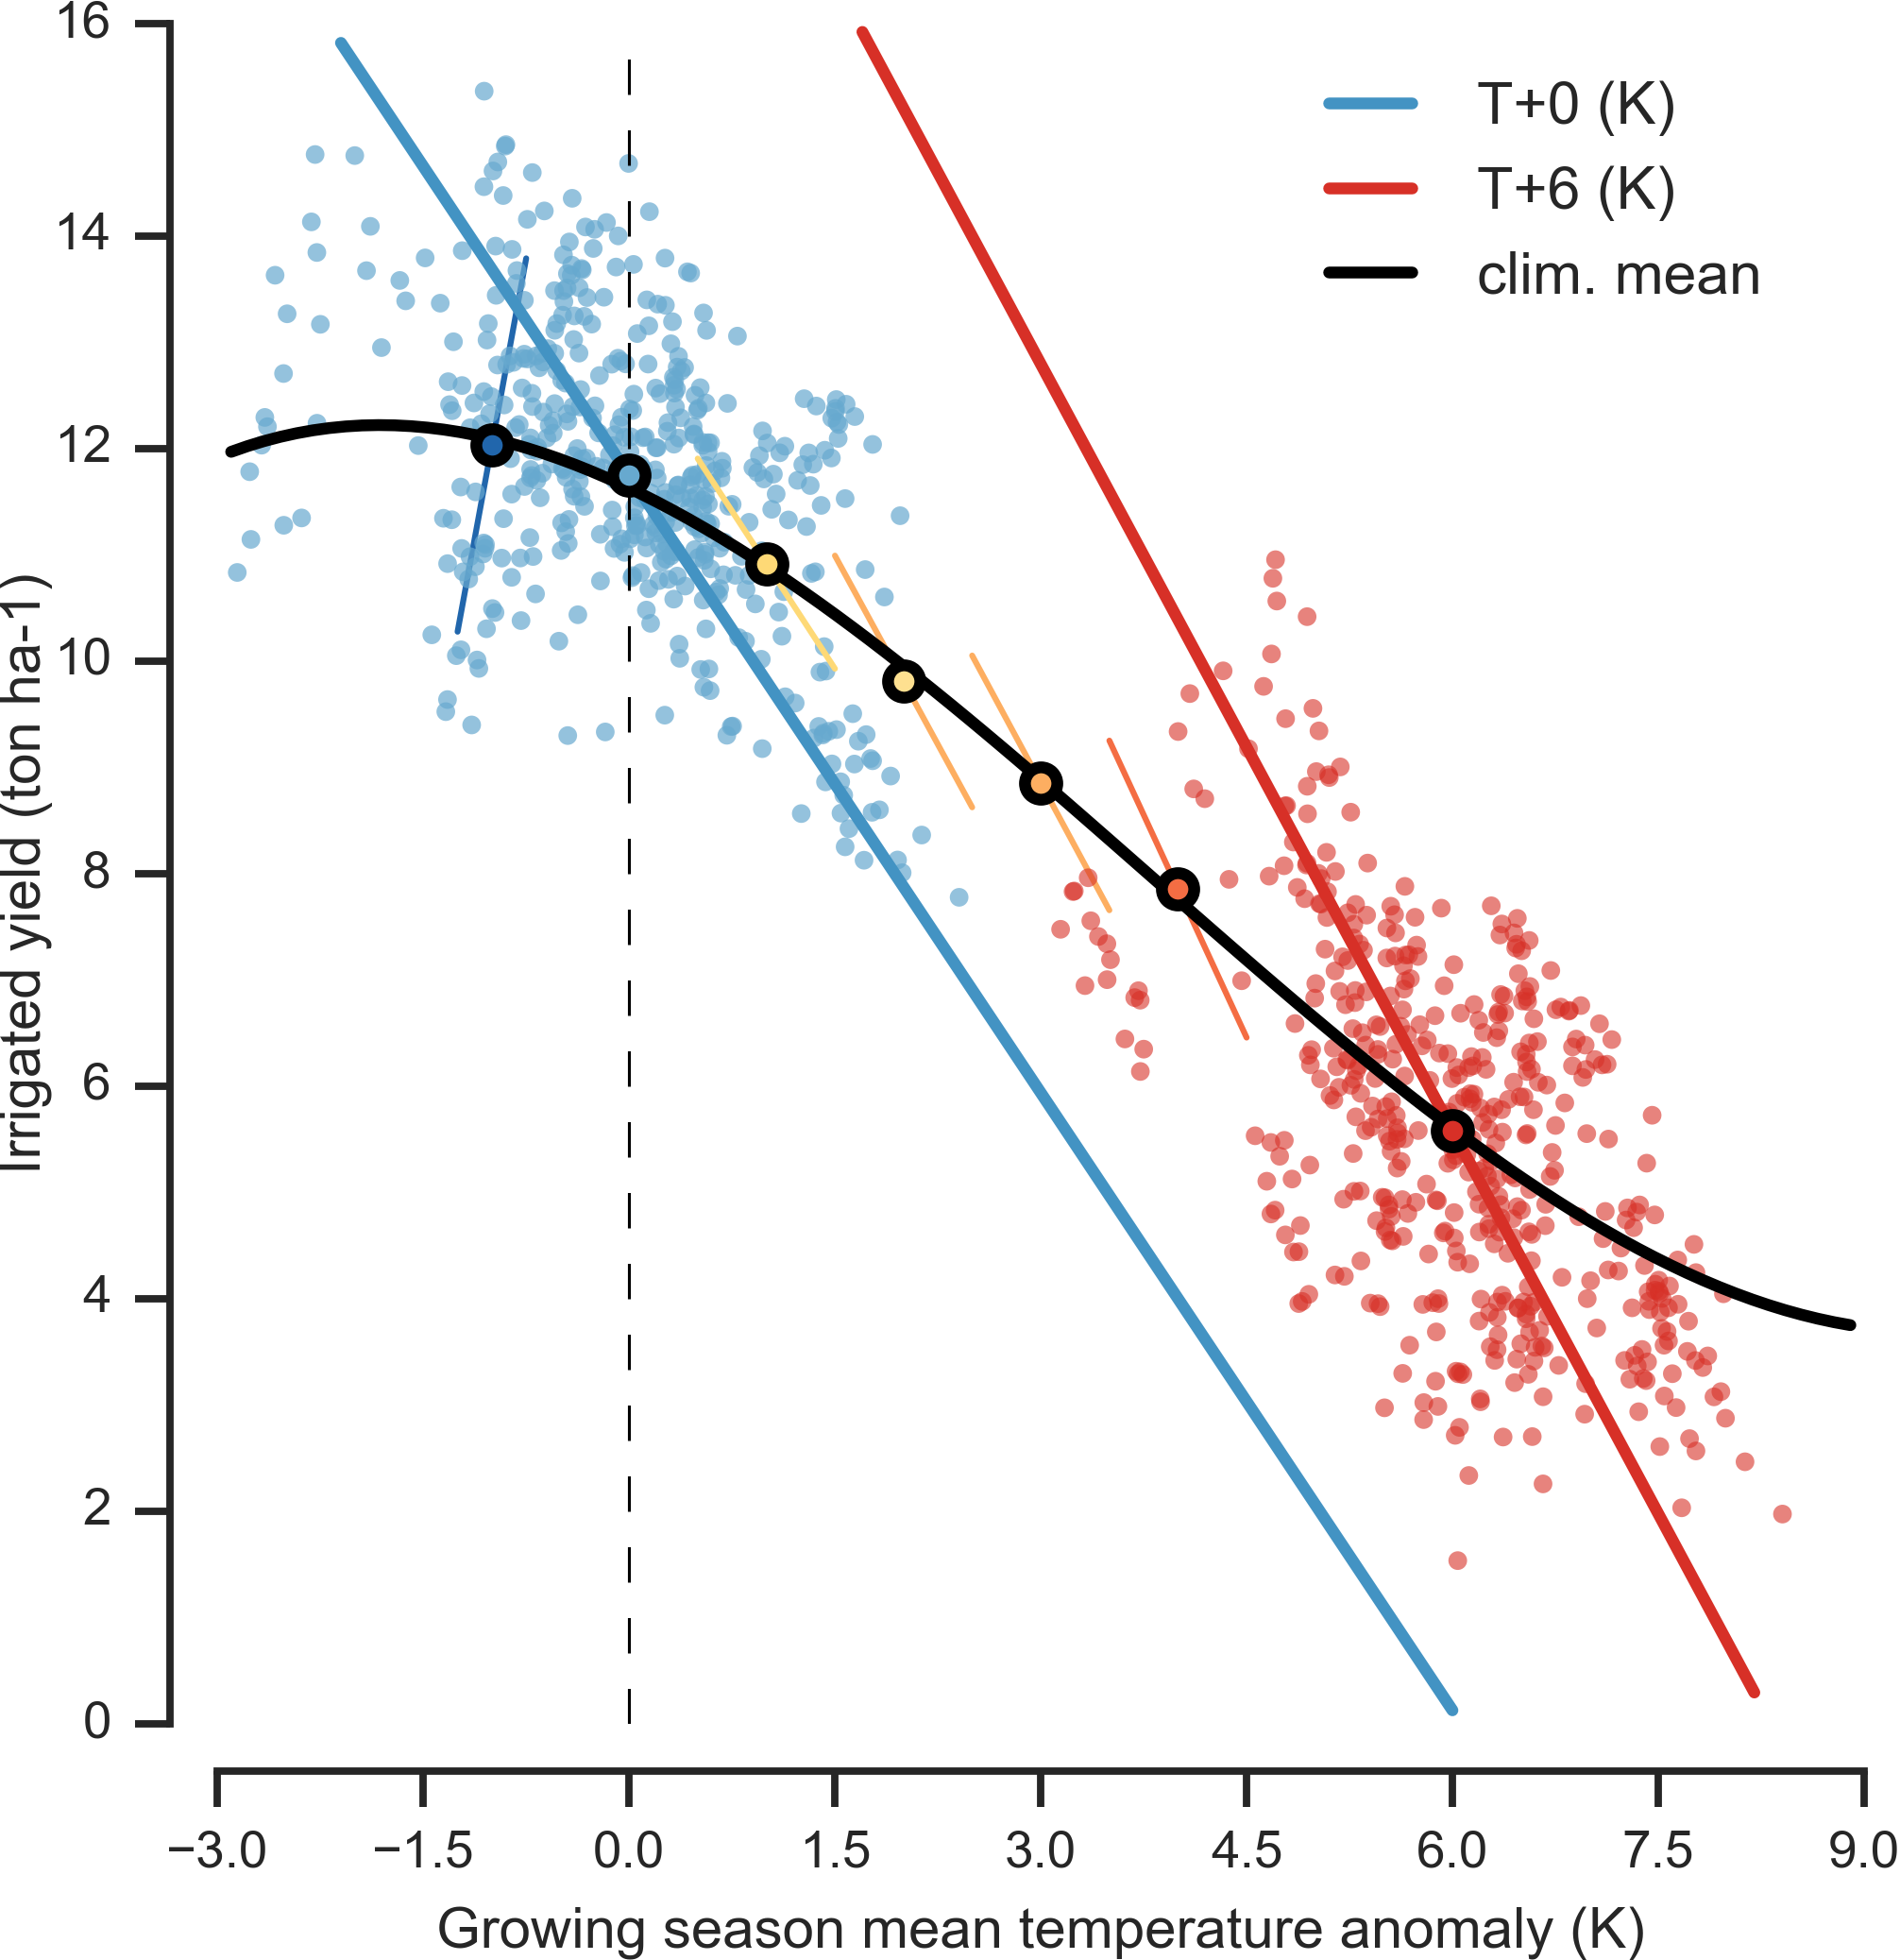
\includegraphics[width=8.3cm]{figures/tempyearvclim.png}
   \caption{Example showing distinction between crop yield responses to year-to-year and climatological mean temperature shifts. 
   Figure shows irrigated maize for a representative high-yield region (nine adjacent grid cells in northern Iowa) from the pDSSAT model, for the baseline 1981-2010 historical climate (blue) and for the scenario of maximum temperature change (+6 K, red). Other variables are held at baseline values, and the choice of irrigated yields means that precipitation is not a factor. 
   Open black circles mark climatological mean yield values for all six temperature scenarios (T-1, +0, +1, +2, +3, +4, +6). Colored lines show total least squares linear regressions of year-over-year variations in each scenario. 
   Black line shows the fit through the climatological mean values.  
   Responses to year-over-year temperature variations (colored lines) are 100--200\% larger than those to long-term climate perturbations, rising under warmer conditions. Linear fits are shown for illustration purposes and are not used in the emulation models.}
   \label{fig:yearvclim}
\end{figure}

\begin{figure}[ht]
\centering
   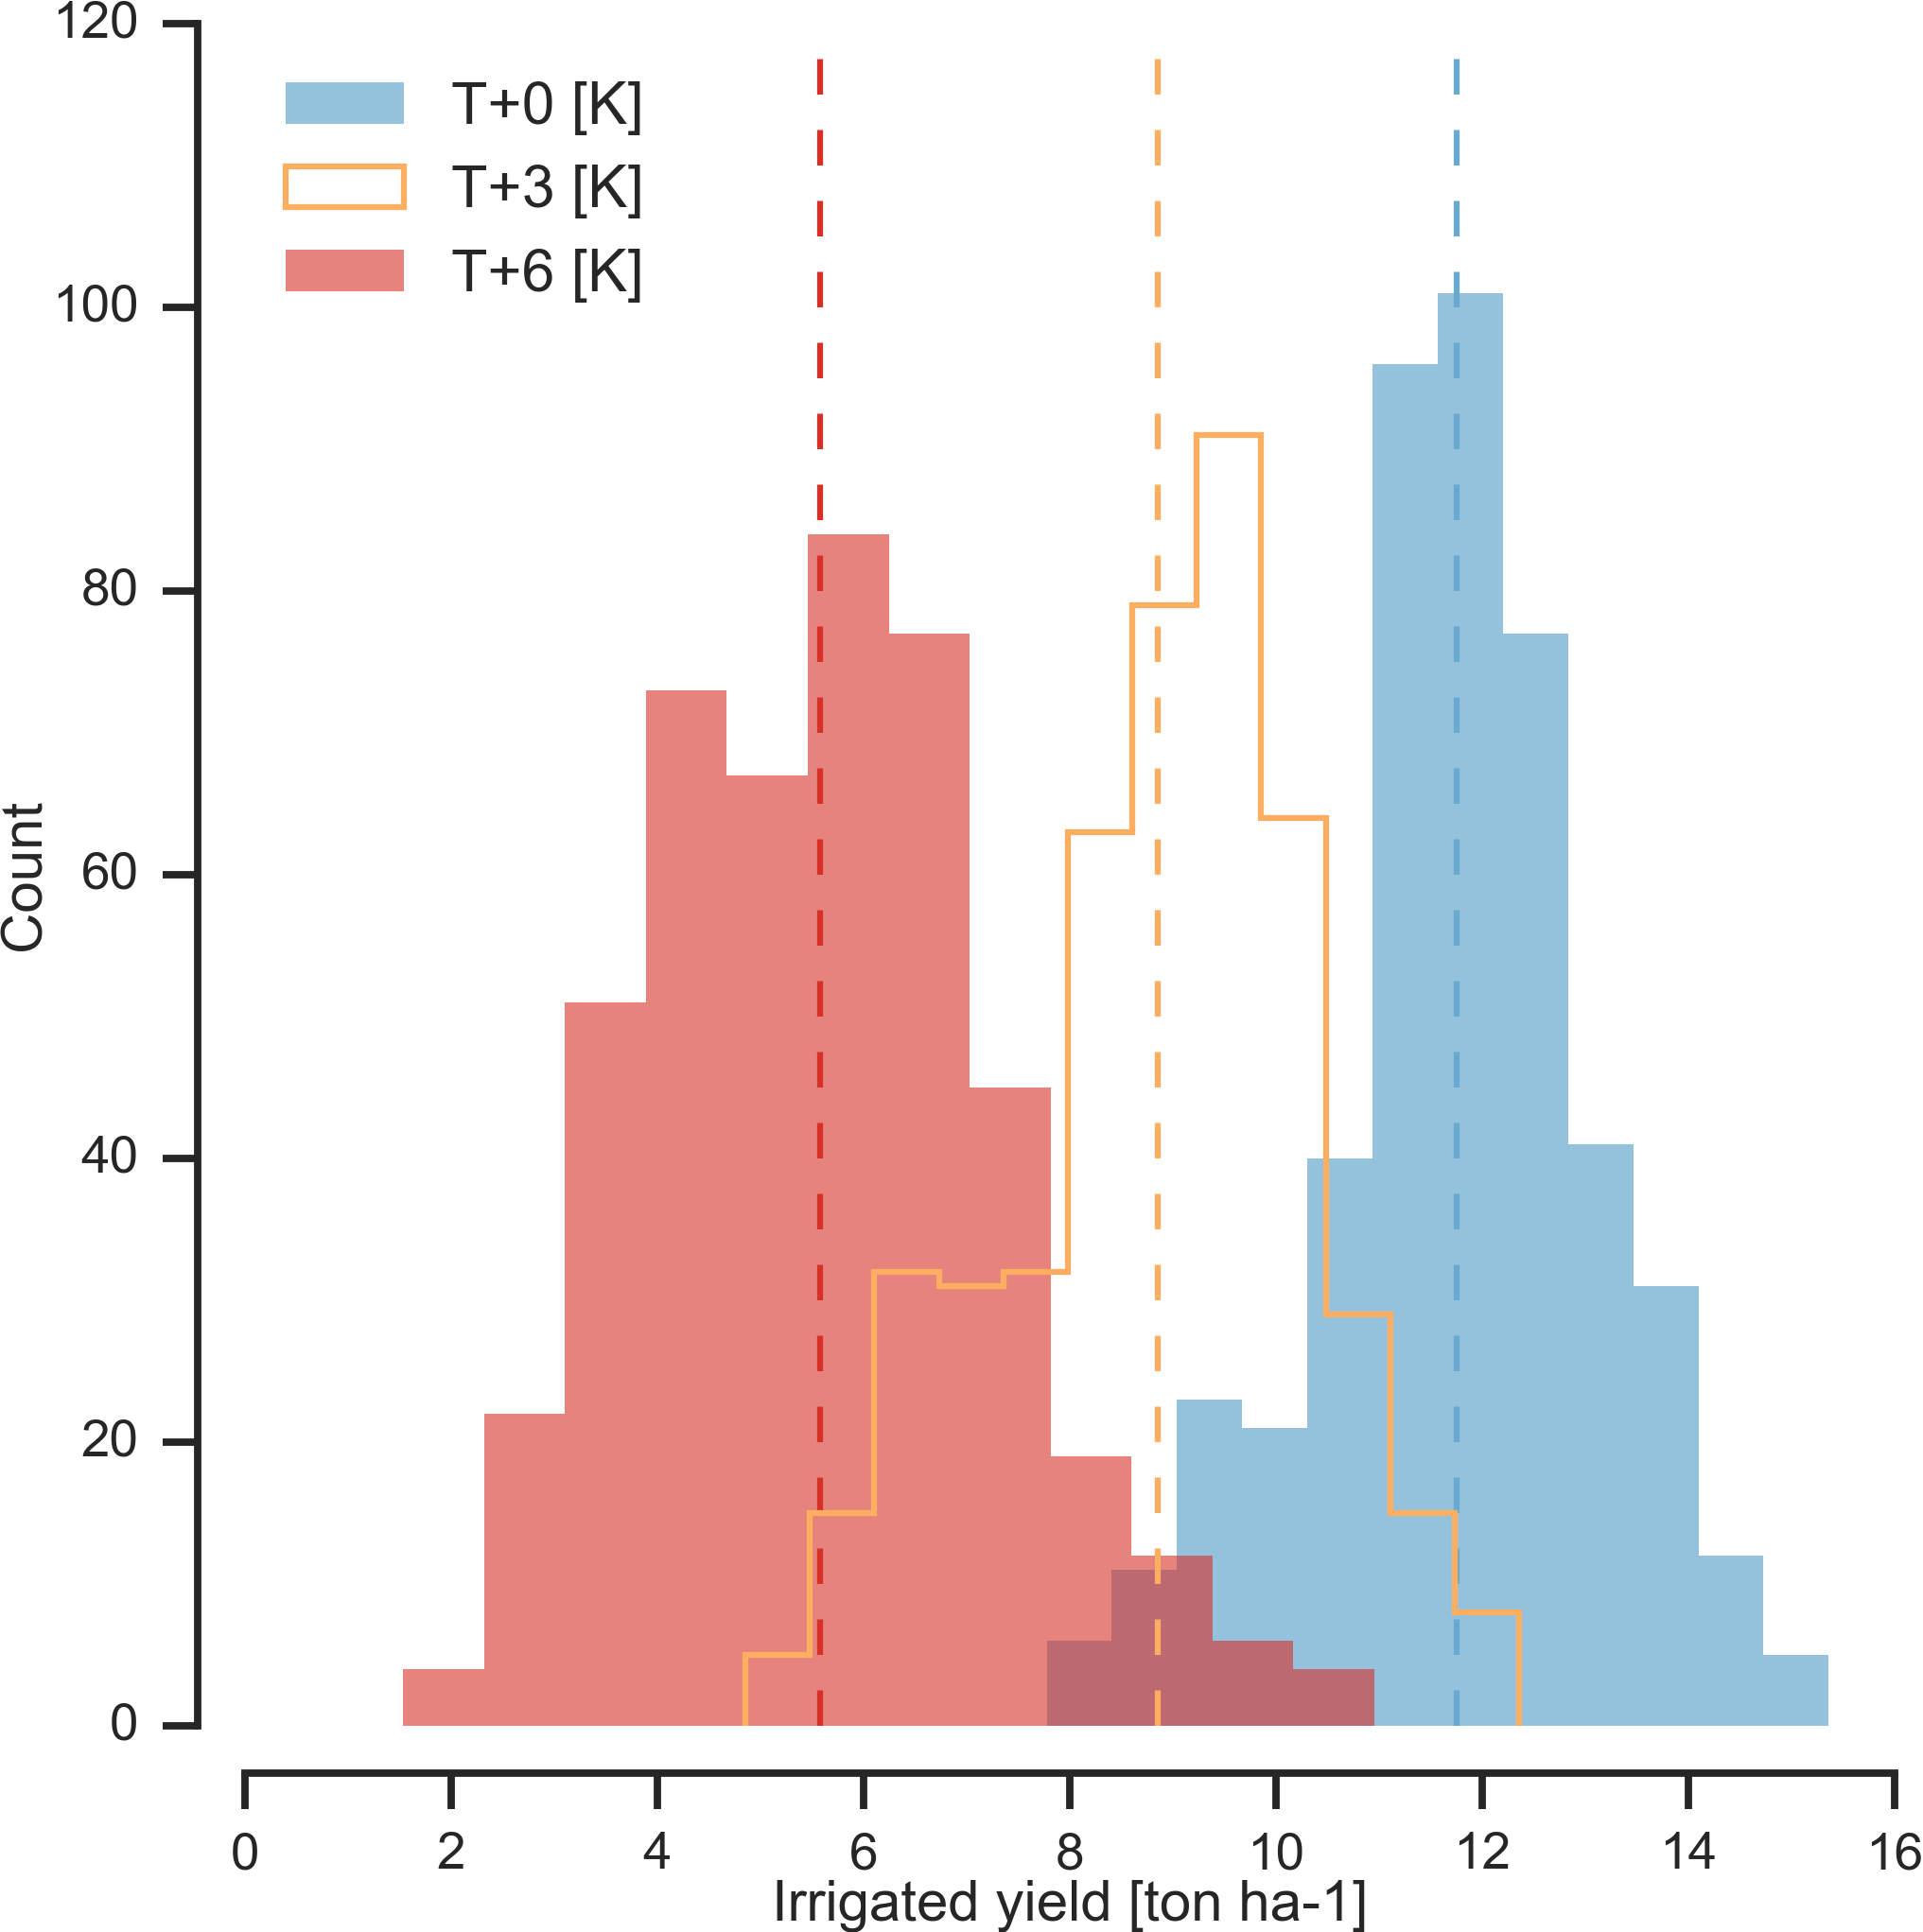
\includegraphics[width=8.3cm]{figures/hist_year.png}
   \caption{Example showing climatological mean yields and distribution of yearly yields for three 30-year scenarios. 
   Figure shows irrigated maize for nine adjacent high-yield grid cells of Figure \ref{fig:yearvclim} from the pDSSAT model, for the baseline 1981-2010 historical climate (blue) and for scenarios with temperature shifted by T+3 (orange) and T+6 K (red), with other variables held at baseline values. 
   The stronger year-over-year temperature response with higher temperatures seen in Figure \ref{fig:yearvclim} is manifested here as larger variance in annual yields even though the variance in climate drivers is identical. 
   In this work we emulate not the year-over-year distributions but the climatological mean response (dashed vertical lines).}
   \label{fig:yearly}
\end{figure}

\begin{figure}[ht]
\centering
   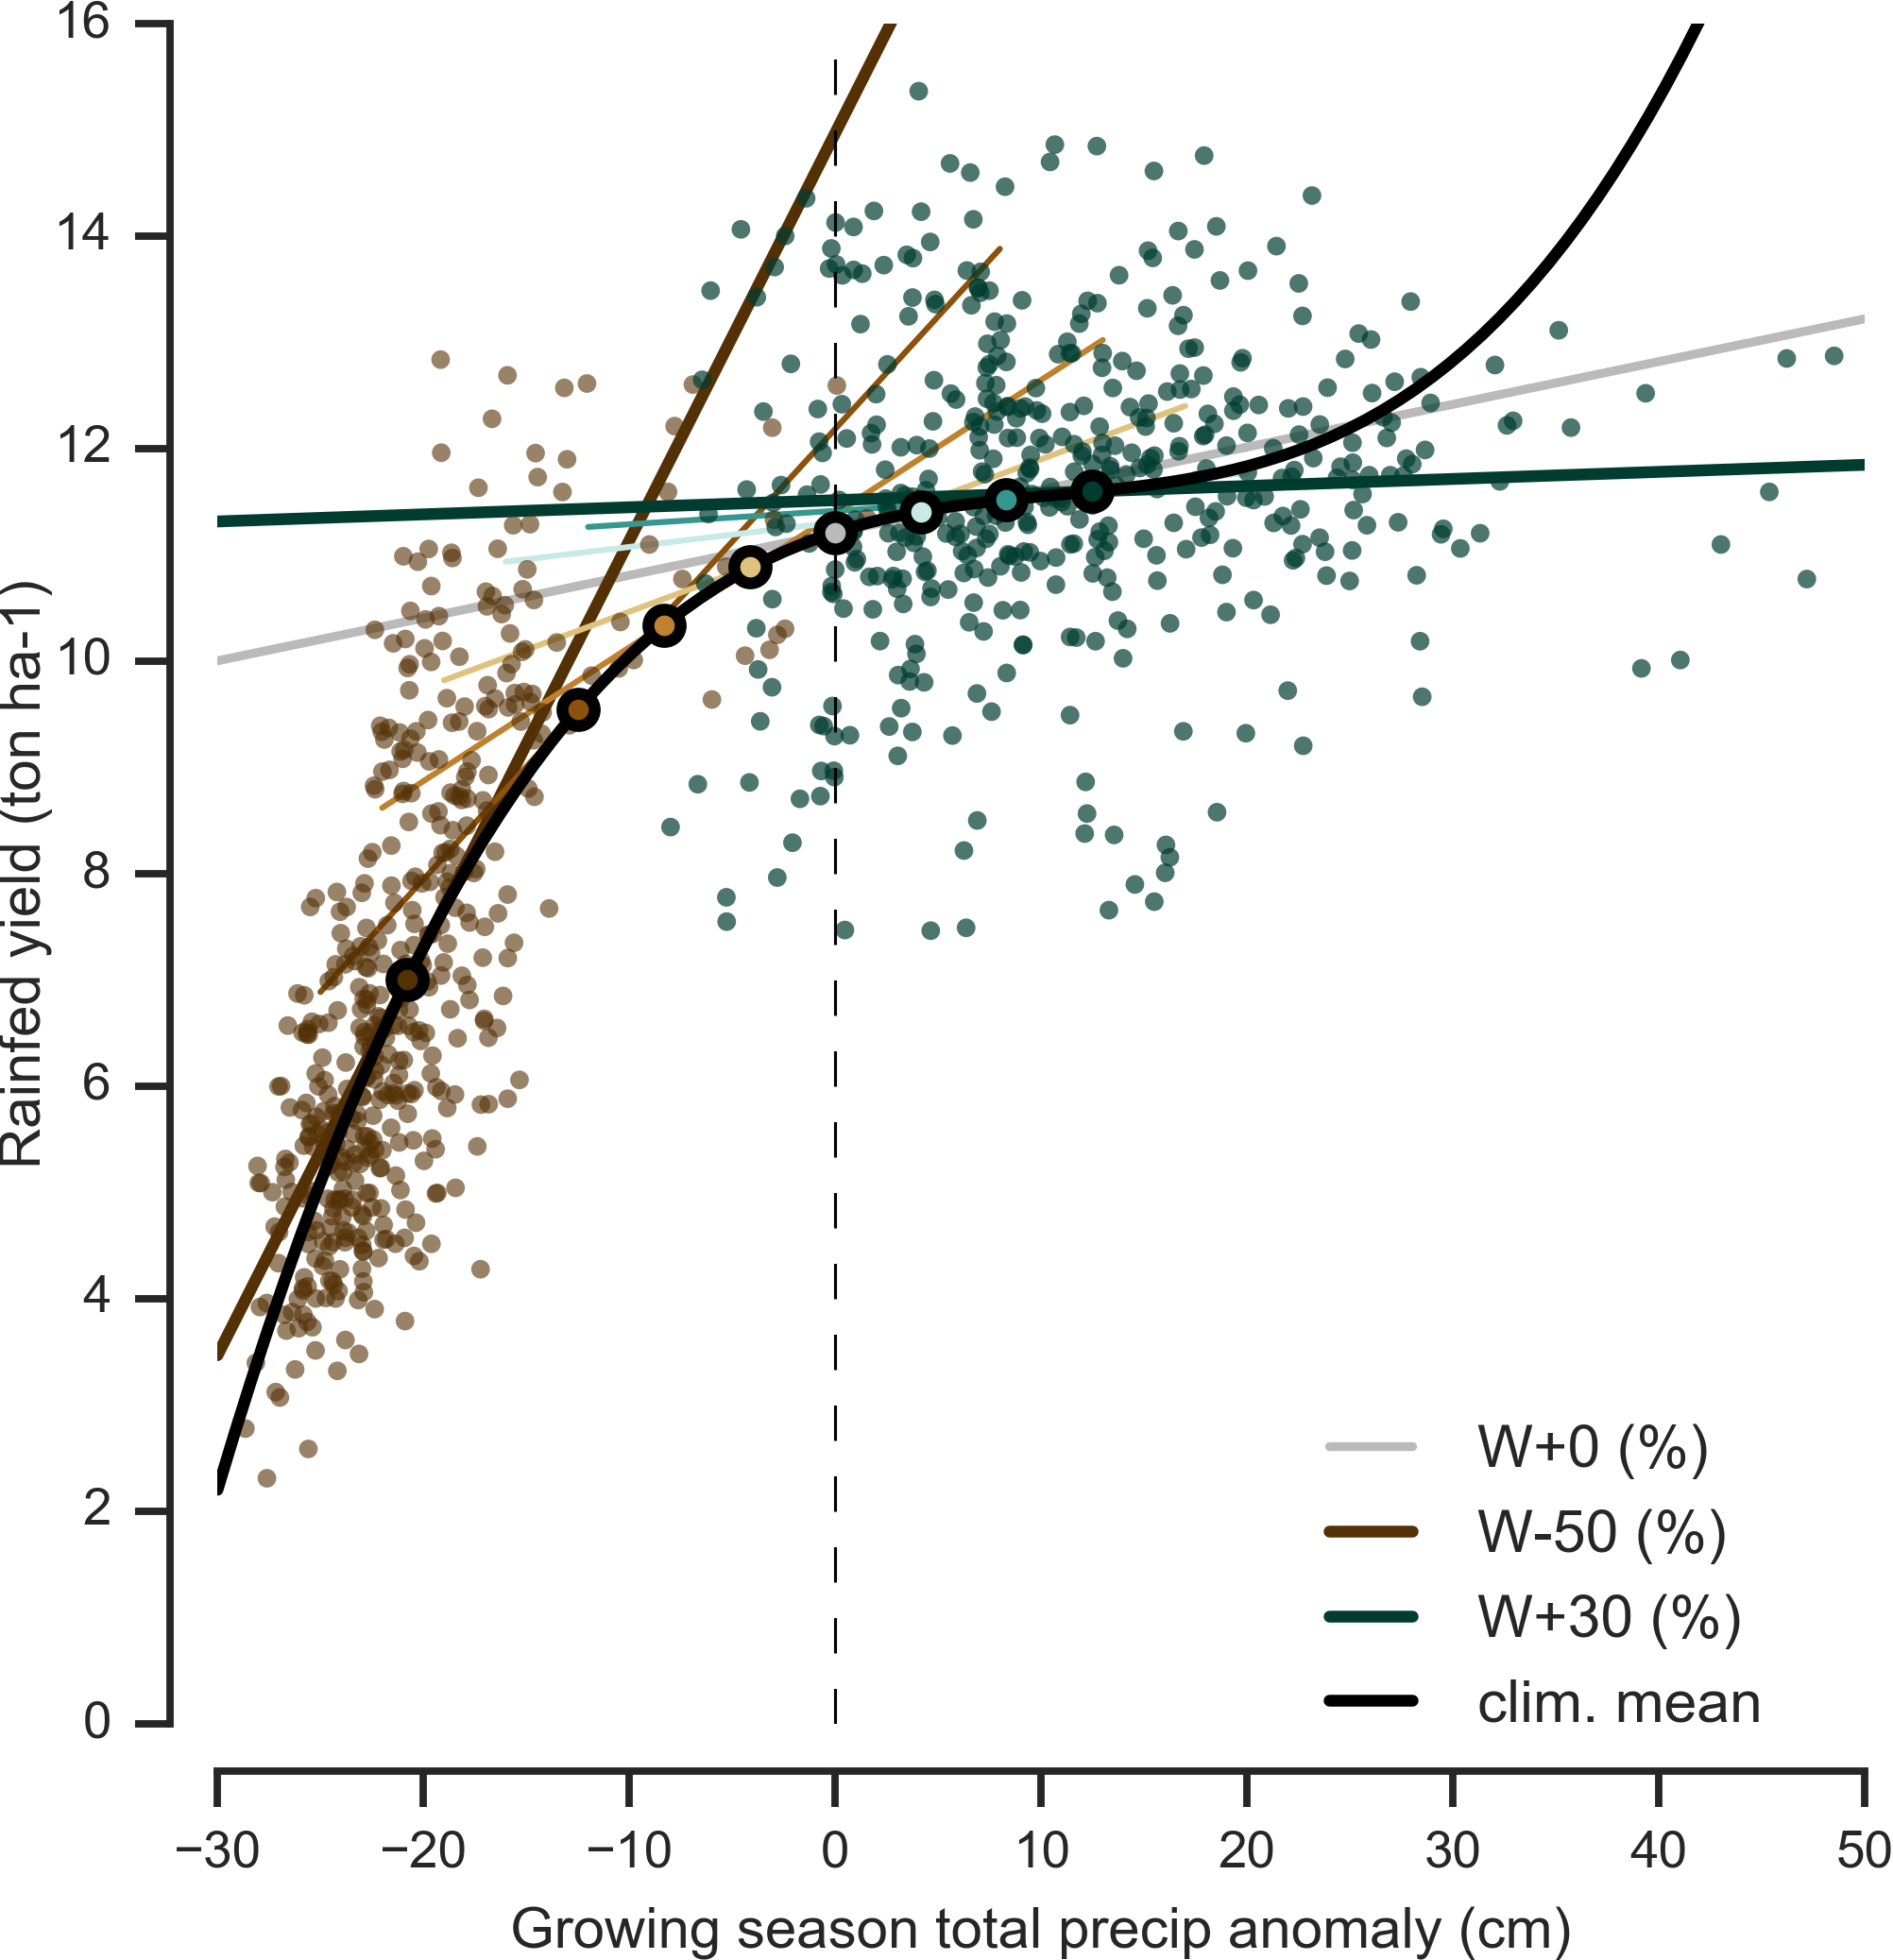
\includegraphics[width=8.3cm]{figures/pryearvclim.png}
   \caption{Example showing distinction between crop yield responses to year-to-year and climatological mean precipation shifts. 
   Figure shows raifed maize for a representative high-yield region (nine adjacent grid cells in northern Iowa) from the pDSSAT model, for the baseline 1981-2010 historical climate (gray) and for the scenario of maximum and minimum precip change (brown and green). 
   Other variables are held at baseline values, and the choice of irrigated yields means that precipitation is not a factor. 
   Open black circles mark climatological mean yield values for all six temperature scenarios (T-1, +0, +1, +2, +3, +4, +6). 
   Colored lines show total least squares linear regressions of year-over-year variations in each scenario. 
   Black line shows the fit through the climatological mean values. 
   Linear fits are shown for illustration purposes and are not used in the emulation models.}
   \label{fig:yearvclim}
\end{figure}

As most assessment models project impacts at some large temporal scale (decades) or utilize some temporally aggregated climate projection, we construct an emulator of 30-year climatological mean yields. 
This approach is made possible by the structured set of simulations involving systematic perturbations. 
In the GGCMI Phase II dataset, the year-over-year responses are generally quantitatively distinct from (and larger than) climatological mean responses. 
In the example Figure \ref{fig:yearvclim}, responses to year-over-year temperature variations are 100\% larger than those to long-term perturbations in the baseline case, and larger still under warmer conditions, rising to nearly 200\% more in the T+6 case. 
The stronger year-over-year response under warmer conditions also manifests as a wider distribution of yields (Figure \ref{fig:yearly}). 
As discussed previously, year-over-year and climatological responses can differ for many reasons including memory in the crop model, lurking covariants, and differing associated distributions of daily growing-season daily weather \citep[e.g.][]{Ruane2016}. 
Note that the GGCMI Phase II datasets do not capture one climatological factor, potential future distributional shifts, because all simulations are run with fixed offsets from the historical climatology. 
Prior work has suggested that mean changes are the dominant drivers of climatological crop yield shifts in non-arid regions \citep[e.g.][]{Glotter14}. 

Emulation involves fitting individual regression models for each crop, simulation model, and 0.5 degree geographic pixel from the GGCMI Phase II dataset; the regressors are the applied constant perturbations in CO$_2$, temperature, water, and nitrogen (C,T, W, N).  
We regress 30-year climatological mean yields against a third-order polynomial in C, T, W, and N with interaction terms. 
We aggregate the entire 30-year run in each case to improve signal to noise ratio. 
The higher-order terms are necessary to capture any nonlinear responses, which are well-documented in observations for temperature and water perturbations (e.g.\ \citet{Schlenker2009} for T and \citet{He2016} for W). 
We include interaction terms (both linear and higher-order) because past studies have shown them to be significant effects. 
For example, \citet{Lobell2007} and \citet{Tebaldi2008} showed that in real-world yields, the joint distribution in T and W is needed to explain observed yield variance. 
(C and N are fixed in these data.) 
Other observation-based studies have shown the importance of the interaction between water and nitrogen \citep[e.g.][]{AULAKH2005}, and between nitrogen and CO$_2$ \citep{Mitsuru92, Nakamura97}. 
To avoid over-fitting or unstable parameter estimation, we apply a feature selection procedure (described below) that reduces the potential 34-term polynomial (for the rainfed case) to 23 terms.

We do not focus on comparing different functional forms in this study, and instead choose a relatively simple polynomial parametrization that allows for some interpretation of coefficients. 
Some prior studies have used other statistical specifications, e.g.\ 39 term fractional polynomial in \citet{BLANC2015} and \citet{BLANC2017}, who borrow information across space by fitting grid points simultaneously across soil region in a panel regression. 
The relativity simple functional form used here allows fast model emulation at the grid cell level as opposed to the global or large regional level. 
The emulation therefore indirectly includes any yield response to geographically distributed factors such as soil type, insolation, and the baseline climate. 
We hold the statistical specification constant across all crops and models to facilitate parameter by parameter simulation model comparison.

%A Gaussian process model was also tested as a potential statical functional form. 
%A Gaussian process model can be fit to the response in a single grid cell, and generally outperforms the polynomial in terms of out of sample prediction, but quickly becomes cumbersome in the context of fitting individual kernels across 40,000 grid cells for a single simulation model and crop.

\begin{figure*}[ht]
\centering
   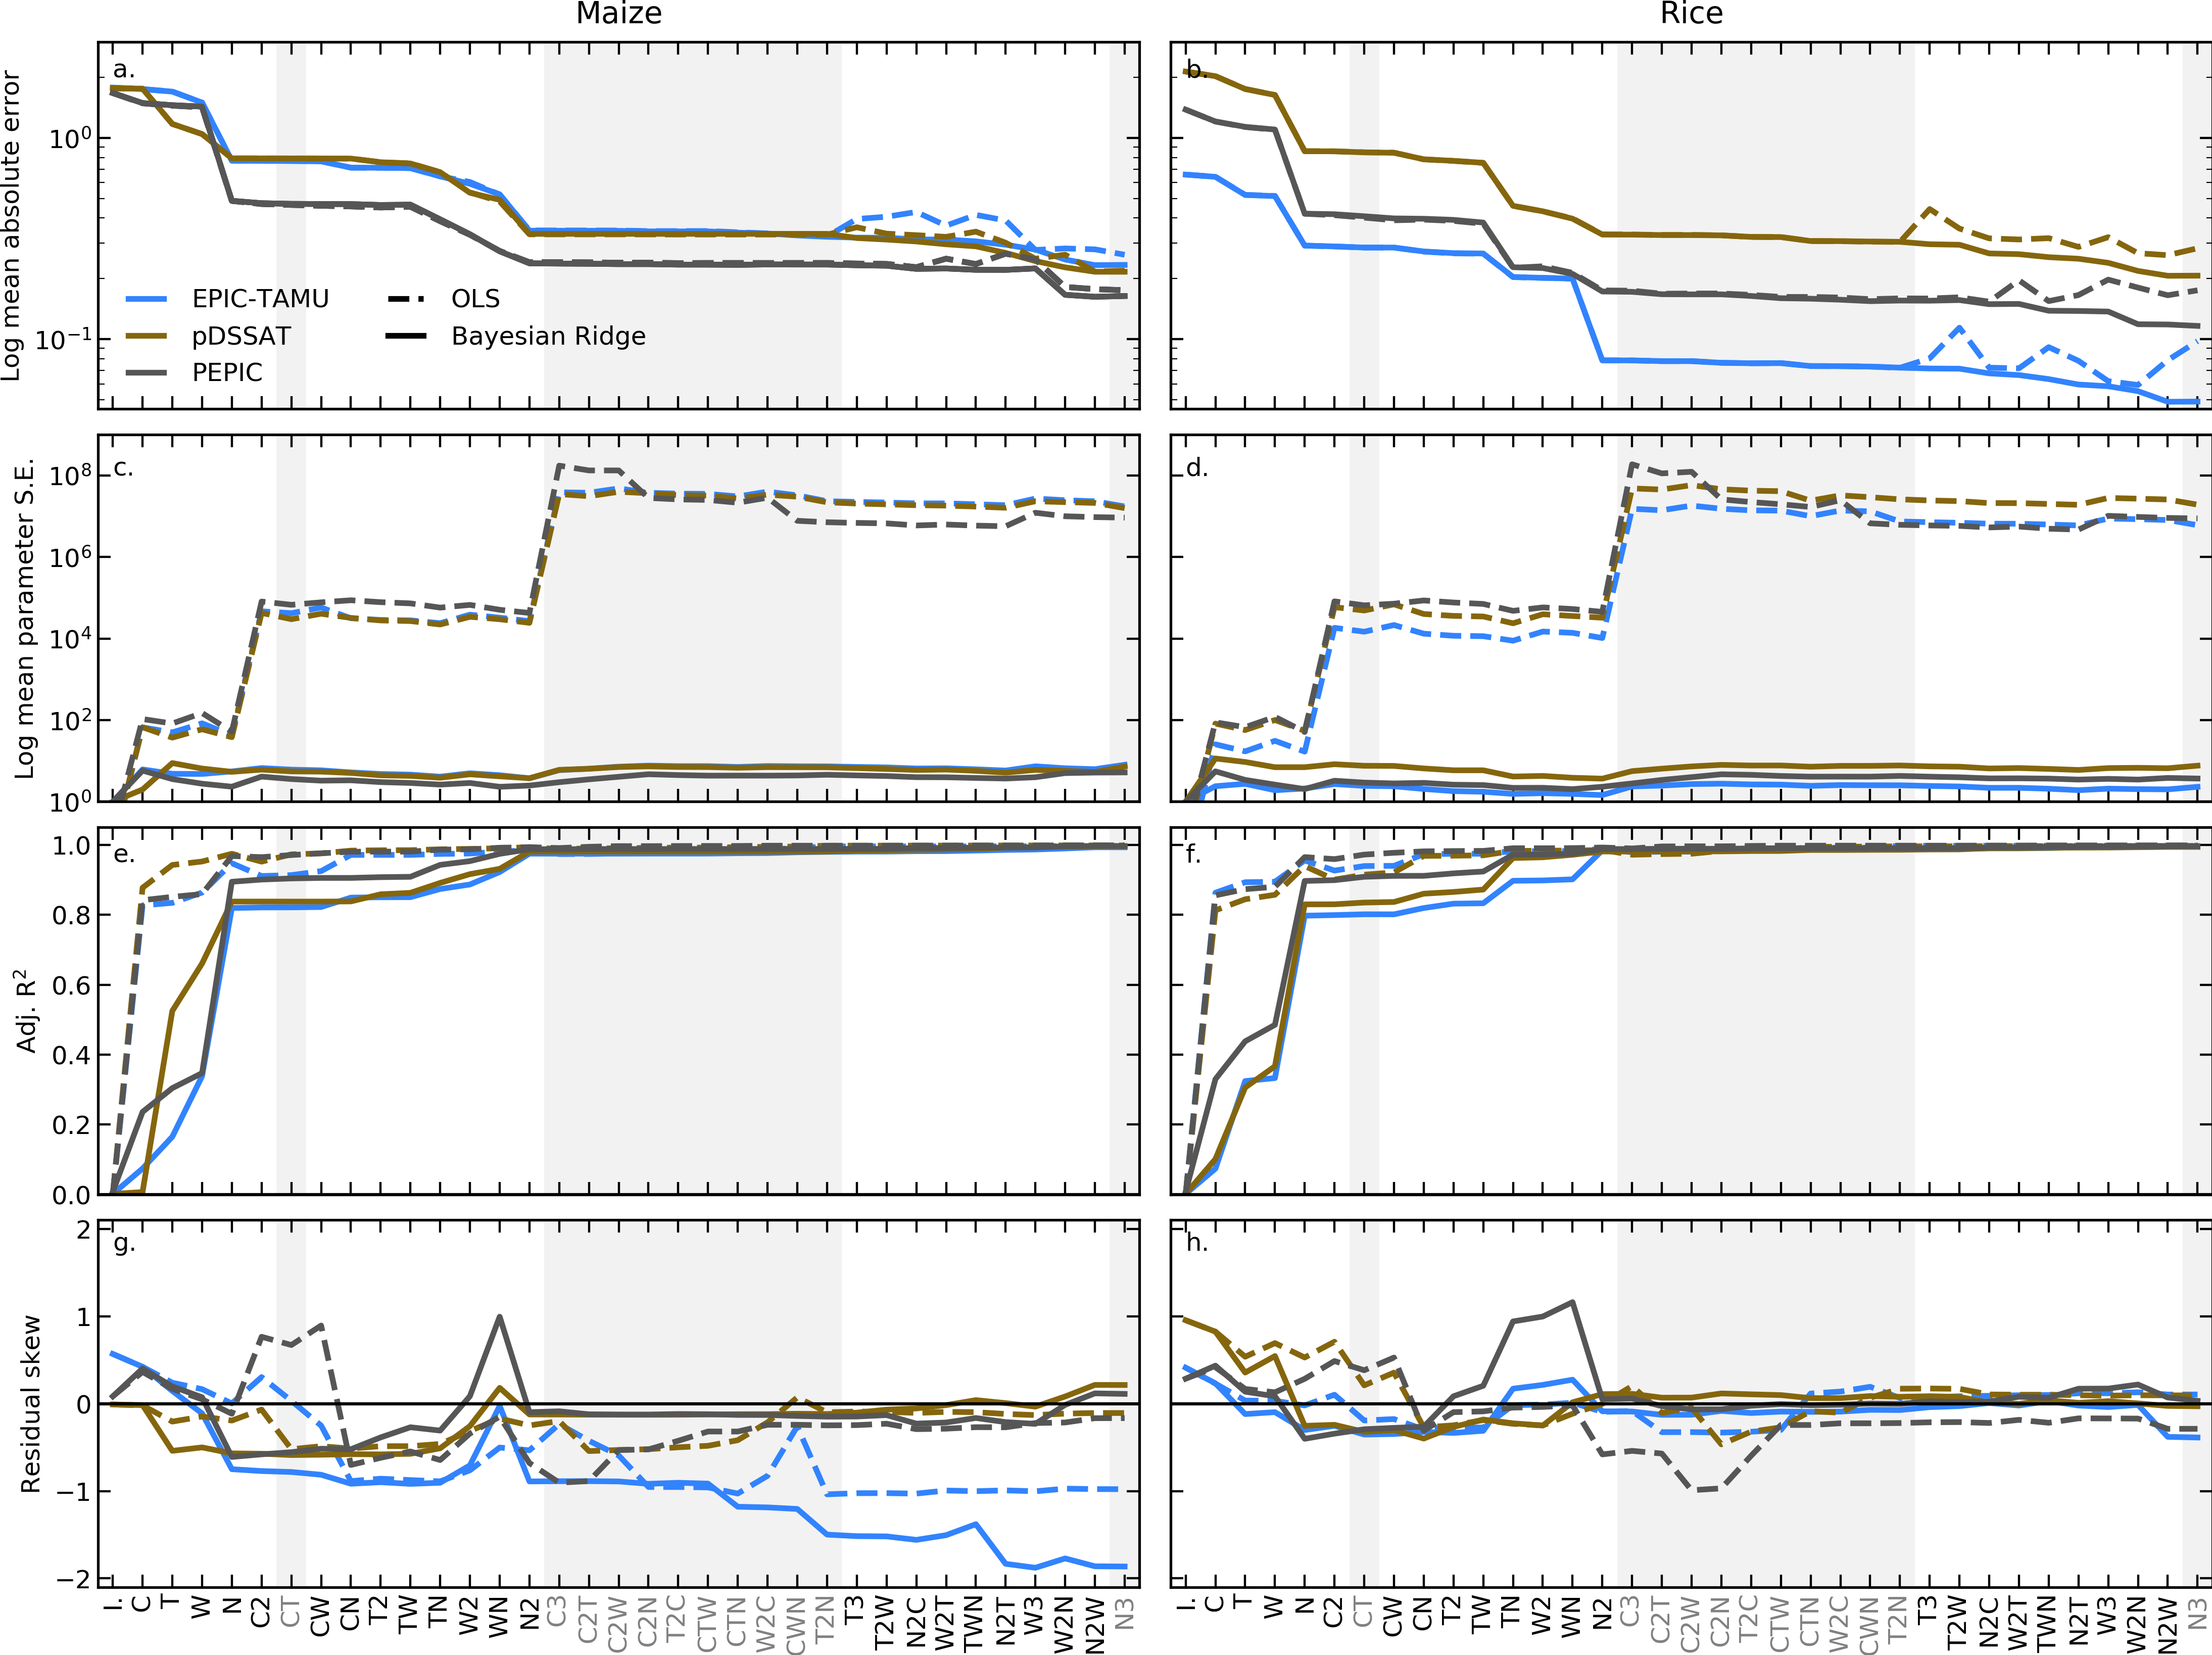
\includegraphics[width=15cm]{figures/model_select_maize_rice.png}
   \caption{Summary results from polynomial feature selection process.
   Top row illustrates log mean absolute error between emulated yield and simulated values calucled from a three fold cross validation process, where the emulator is trained on two thirds of the data and predicts the remaining third.
   The second row illustrates the adjusted R$^2$ score for the fit at each model specification where additionally terms are penalized.
   The third row illustrates the log mean standard parameter error and the forth and fifth rows illustrate the distribution of the residuals.
   The X- axis indicates terms included in the model at each step progressively where T = temperature, T2 = temperature$^{2}$, TW  = temperature * water and so on. 
   The terms that did not reduce the aggregate error (horizontal lines) are not included in the final model. 
   Solid lines indicate Bayesian Ridge regression results and dashed lines indicated standard ordinary least squares. 
   Colors indicated three different models.}
   \label{fig:features}
\end{figure*}

Although the GGCMI Phase II sampled variable space is relatively large, it is still sufficiently limited that use of the full polynomial expression described above can be problematic. 
We therefore reduce the number of terms through a feature selection cross-validation process in which terms in the polynomial are tested for importance. 
In this procedure higher-order and interaction terms are added successively to the regression model one by one. 

We then calculate an aggregate mean absolute error with each increasing terms and eliminate those terms that do not contribute significant reductions (Figure \ref{fig:features}). 
Some terms that did not reduce the aggregate error are included if a higher order version of that term provided a decrease in mean squared error (i.e. temperature cubed cannot be included without the temperature squared term, and the linear temperature term). 
We select terms by applying the feature selection process to three example models: two that provided the complete set of 672 rainfed simulations (pDSSAT, EPIC-TAMU, and one that provided the smallest training set 130 (PEPIC). The resulting choice of terms is then applied for all emulators and all crops. 
There is some heterogeneity of parameter 
Since the goal of the emulator is interpolation within the sample space and not extrapolation, we air on the side of including terms that are useful in at least some cases, because the added predictive ability outweighs the costs to distribution of the residuals or over fitting.  

Feature importance is remarkably consistent across models (Figure \ref{fig:features}). 
Even though the models exhibit different absolute levels of error, all three models agree remarkably well on feature importance indicated by the terms where the error is reduced and where additional terms provide no predictive benefit (line slopes match in Figure \ref{fig:features}). 
The feature selection process results in a final polynomial in 23 terms, with 11 terms eliminated. 
We omit the N$^3$ term, which cannot be fitted because we sample only three nitrogen levels. 
We eliminate many of the C terms: the cubic, the CT, CTN, and CWN interaction terms, and all higher order interaction terms in C. 
Finally, we eliminate two 2nd-order interaction terms in T and one in W. 
Implication of this choice include that nitrogen interactions are complex and important, and that water interaction effects are more nonlinear than those in temperature. 
The resulting statistical model (Equation \ref{eqn:features_final}) is used for all grid cells, models, and rainfed crops. 
(The regressions for irrigated crops do not contain the W terms and the models that do not sample the nitrogen levels omit the N terms).

\begin{align}
    \label{eqn:features_final}
    Y\ = \ & K_{1}  \\
		+ \ & K_{2}  C     + K_{3}  T     + K_{4}  W     + K_{5}  N   \nonumber \\
		+ \ & K_{6}  C^2   + K_{7}  T^2   + K_{8}  W^2   + K_{9}  N^2 \nonumber \\
		+ \ & K_{10} C W   + K_{11} C N   + K_{12} T W   + K_{13} T N + K_{14} W N \nonumber \\ % lost 1 term, CT
		+ \ & K_{15} T^3   + K_{16} W^3   + K_{17} T W N  \nonumber \\ % lost 2 terms, C^3 and N^3
		+ \ & K_{18} T^2 W + K_{19} W^2 T + K_{20} W^2 N  \nonumber \\ % lost 2 terms, CWN and CTN
		+ \ & K_{21} N^2 C + K_{22} N^2 T + K_{23} N^2 W  \nonumber    % lose 6 terms: T^2N and T^2C, W^2C, 3 C^2 terms
\end{align}

To fit the parameters $K$, we use a Bayesian Ridge probabilistic estimator \citep{MacKay91}, which reduces volatility in parameter estimates when the sampling is sparse, by weighting parameter estimates towards zero. 
The Bayesian Ridge method is necessary to maintain a consistent functional form across all models and locations (see * Table \ref{table:ASE}). 
We use the implementation of the Bayesian Ridge estimator from the scikit-learn package in Python \citep{scikit-learn}. 
In the GGCMI Phase II experiment, the most problematic fits are those for models that provided a limited number of cases or for low-yield geographic regions where some modeling groups did not run all scenarios. 
We do not attempt to emulate models that provided less than 50 simulations. 
The lowest number of simulations emulated across the full parameter space is then 130 (for the PEPIC model). 
The yield output for a single GGCMI Phase II model that simulates all scenarios and all five crops is $\sim$12.5 GB; the emulator is $\sim$100 MB, a reduction by over two orders of magnitude. 

%%%%%%%%%%%%%%%%%%%%%%%%%%%%%%%%%%%%%%%%%%%%%%%%%%%%%%%%%%%%%%%
%%%%%%%%%%%%%%%%%%%%%%%%%%%%%%%%%%%%%%%%%%%%%%%%%%%%%%%%%%%%%%%
%%%%%%%%%%%%%%%%%%%%%%%%%%%%%%%%%%%%%%%%%%%%%%%%%%%%%%%%%%%%%%%
\section{Results}
\label{S:3}

\begin{figure*}[ht]
\centering
    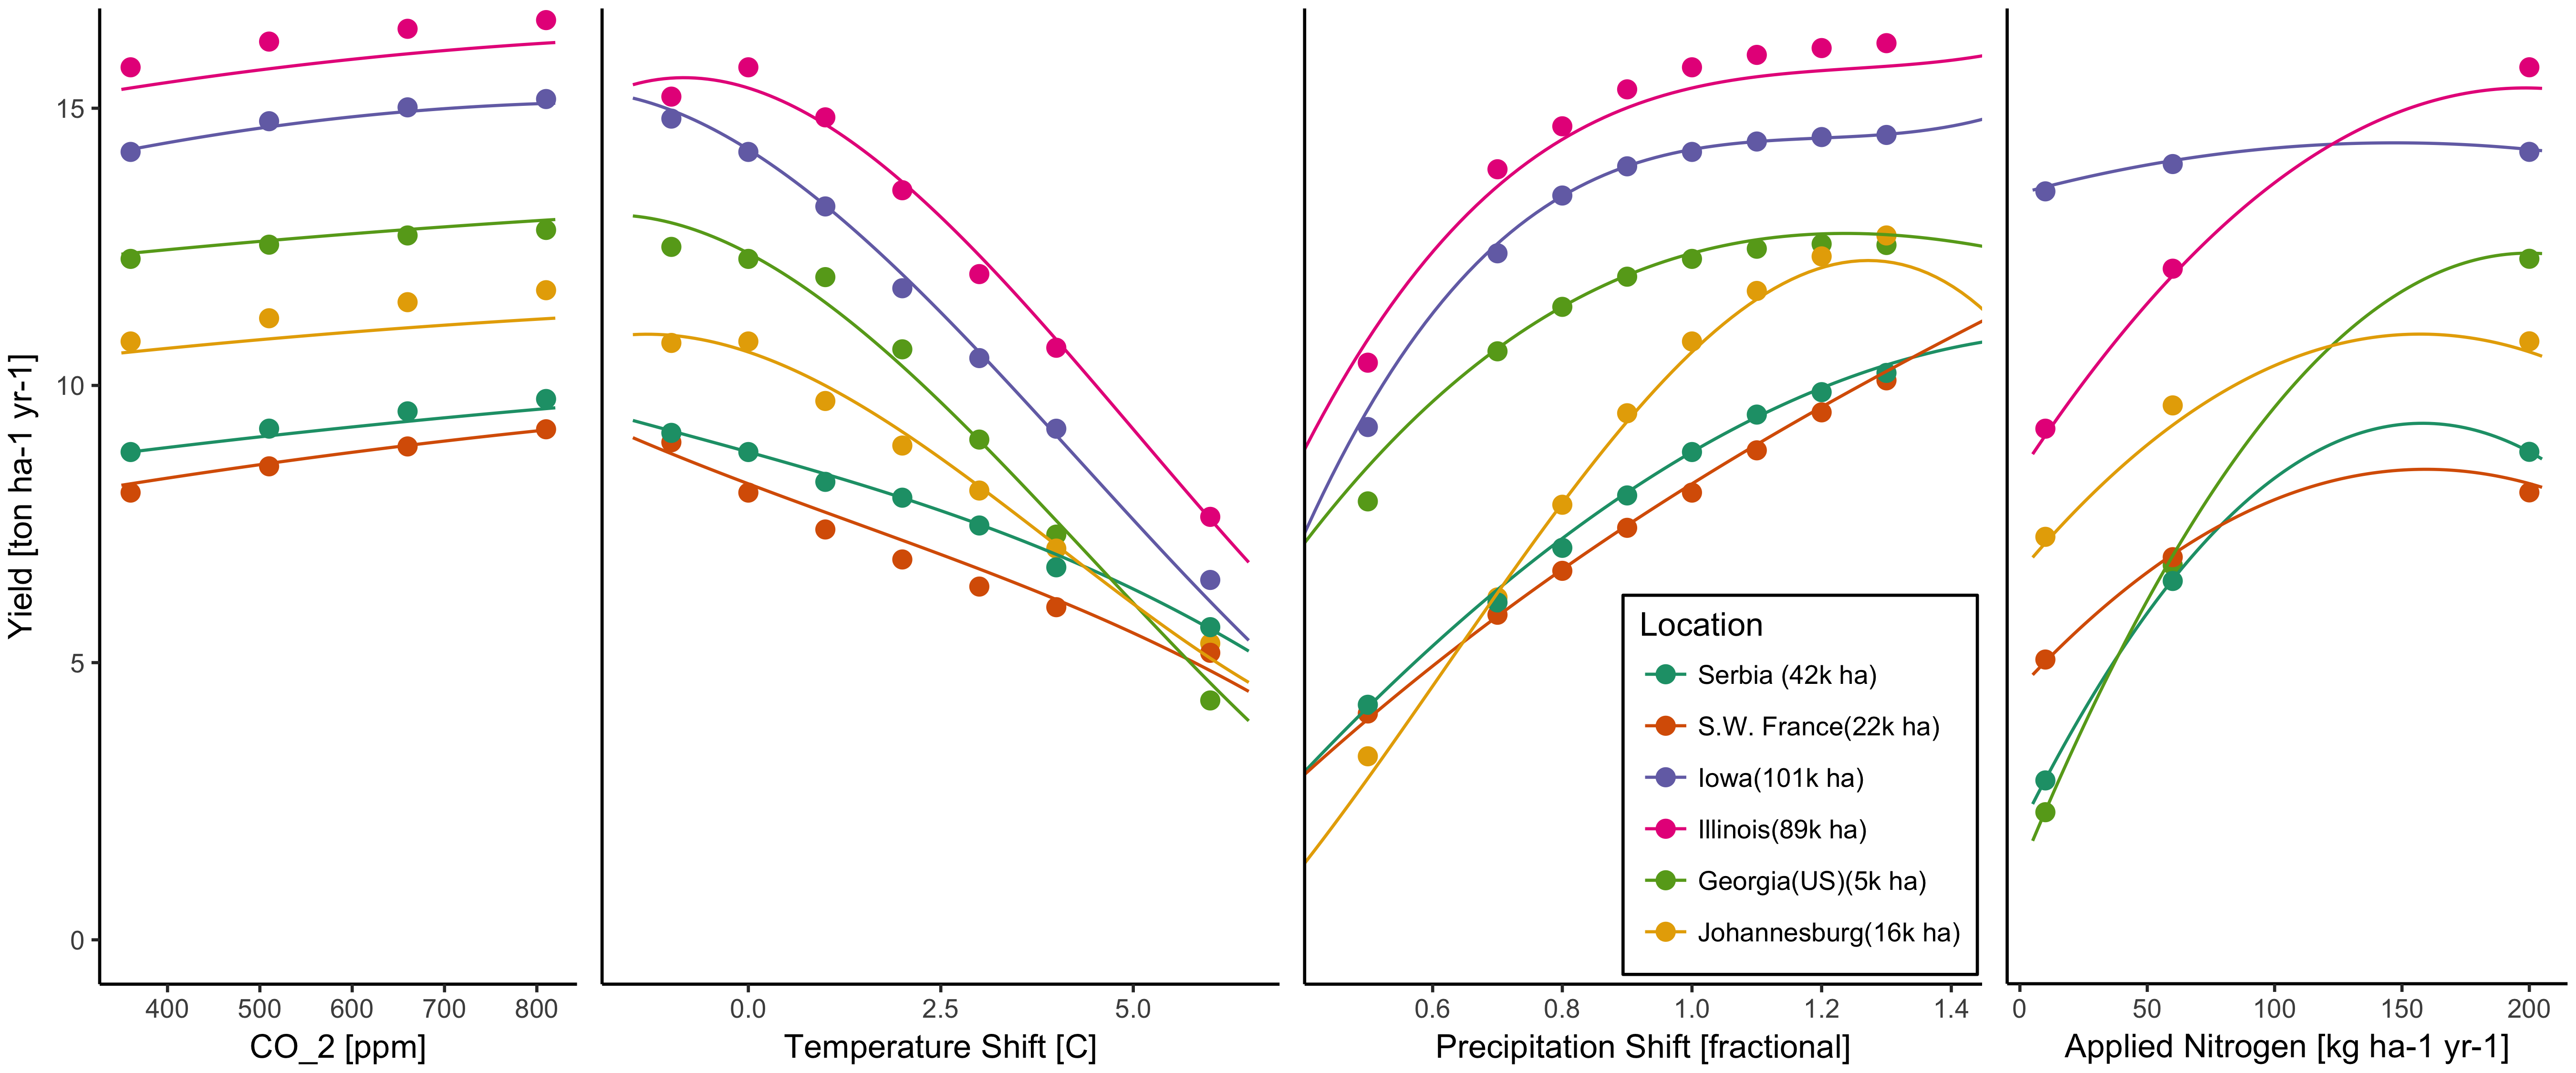
\includegraphics[width=16cm]{figures/regression_areas.png}
    \caption{Illustration of spatial variations in yield response and emulation ability. 
    We show rainfed maize in the pDSSAT model in six example locations selected to represent high-cultivation areas around the globe. 
    Legend includes hectares cultivated in each selected grid cell. 
    Each panel shows variation along a single variable, with others held at baseline values. 
    Dots show climatological mean yields and lines the results of the full 4D emulator of Equation \ref{eqn:features_final}. 
    In general the climatological response surface is sufficiently smooth that it can be represented within the sampled variable space by the simple polynomial used in this work. 
    Extrapolation can however produce misleading results. 
    Nitrogen fits in some cases may not be realistic at intermediate values given limited sampling. 
    For more detailed emulator assessment, see Appendix B.}
   \label{fig:regression}
\end{figure*}

\begin{figure*}[ht]
\centering
    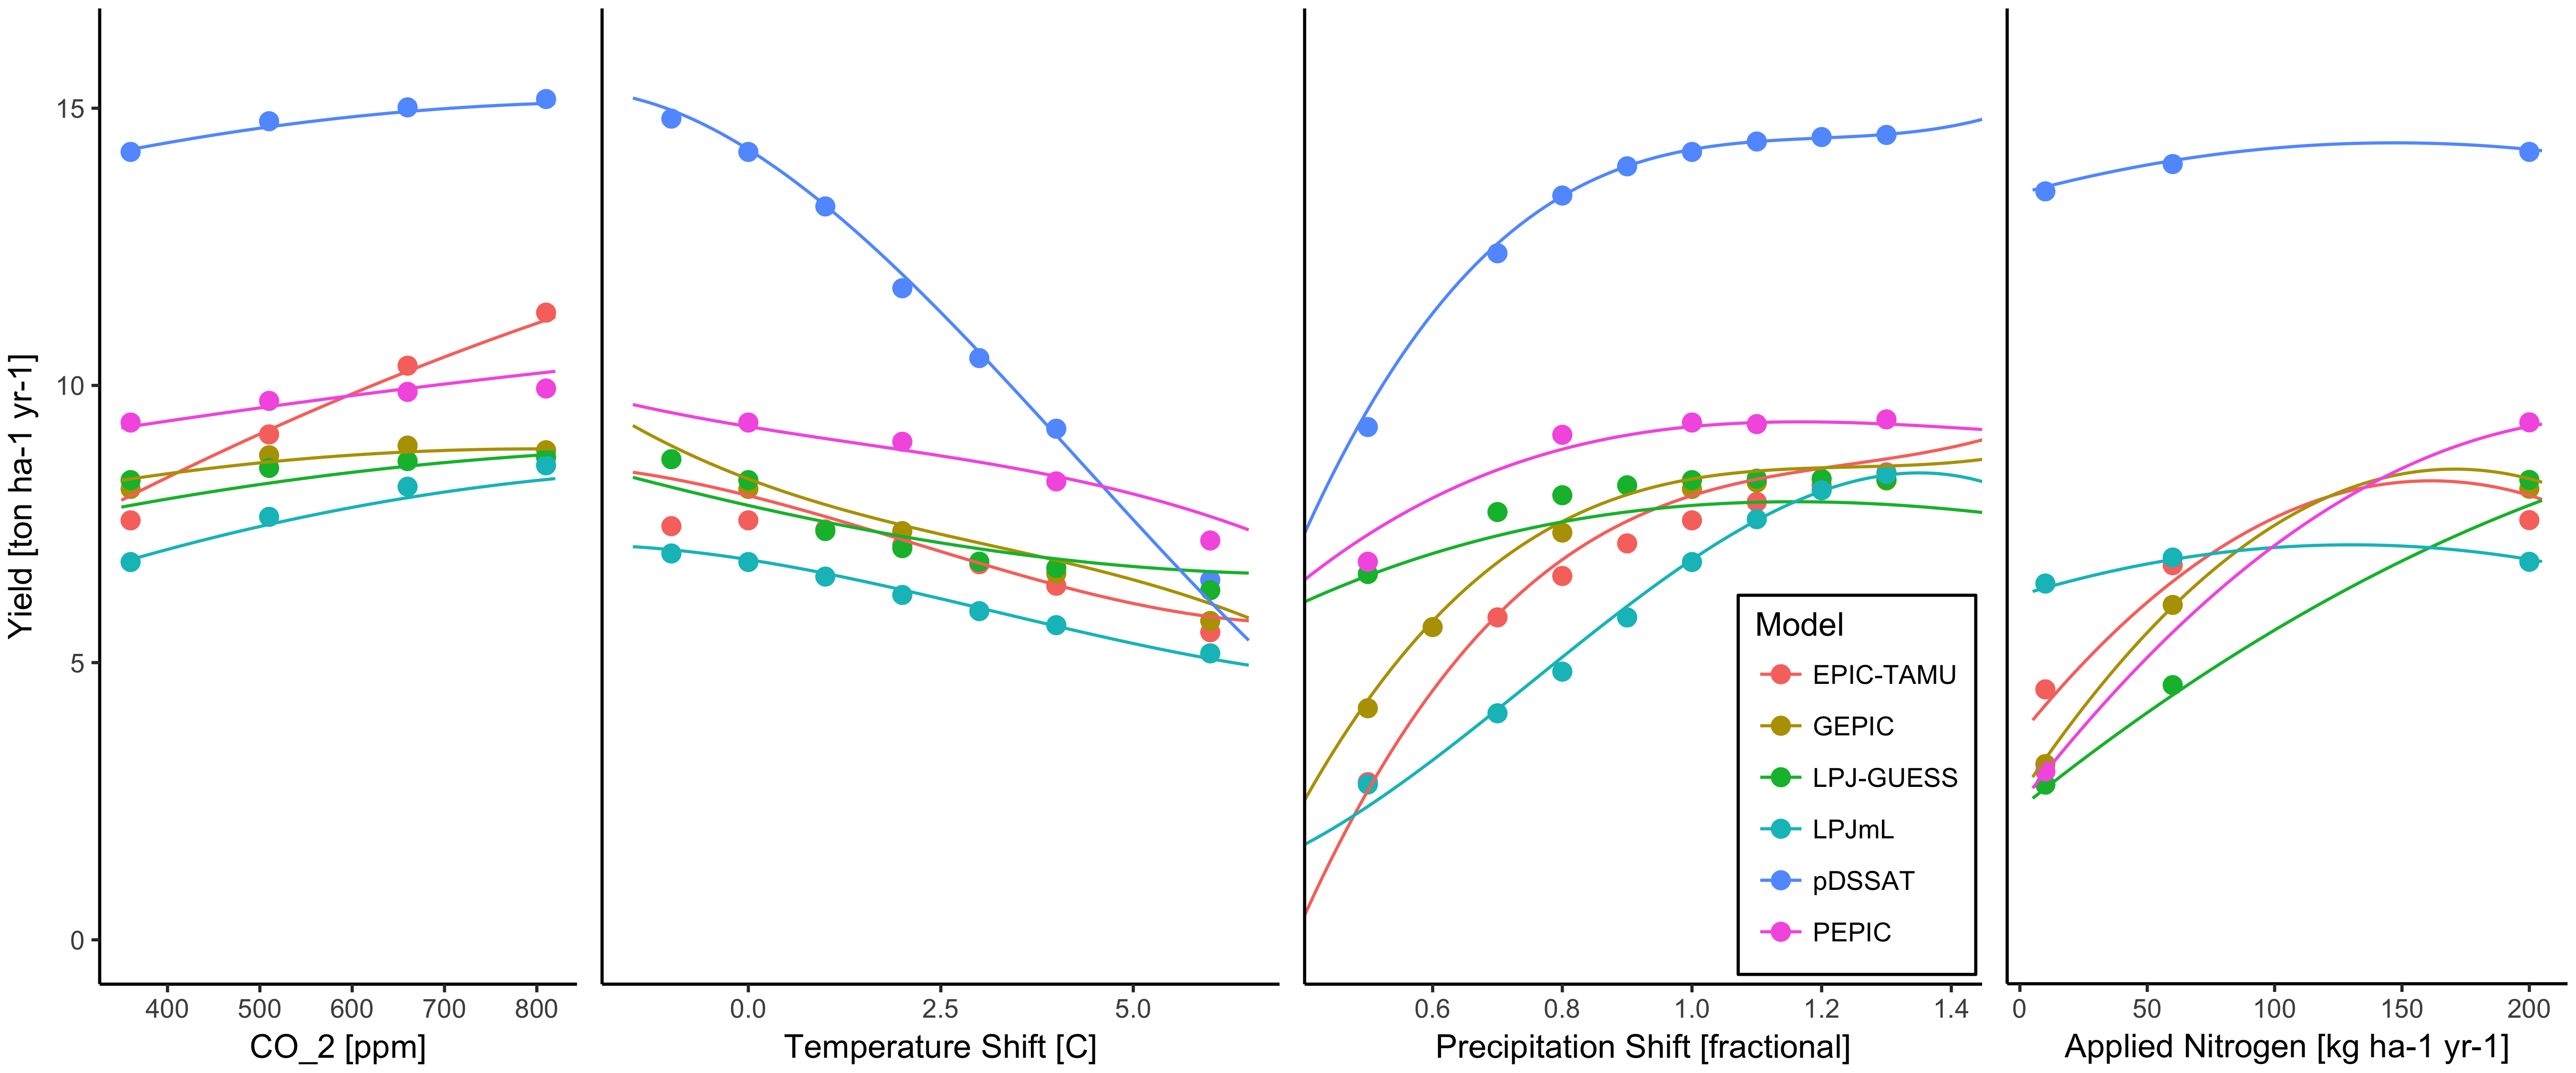
\includegraphics[width=16cm]{figures/regression_model.png}
    \caption{Illustration of across-model variations in yield response. 
    Figures shows simulations and emulations from six models for rainfed maize in the same Iowa grid cell shown in Figure \ref{fig:regression}, with the same plot conventions. 
    Models that do not simulate the nitrogen dimension are omitted for clarity. 
    Note that models are uncalibrated, increasing spread in absolute yields. 
    While most model responses can readily emulated with a simple polynomial, some response surfaces diverge slightly from the polynomial approach (e.g.\ LPJ-GUESS here) and lead to emulation error, though error generally remains small relative to inter-model uncertainty. 
    For more detailed emulator assessment, see Appendix B. 
    As in Figure \ref{fig:regression}, extrapolation out of the sample space is potentially problematic.}
   \label{fig:regression_iowa}
\end{figure*}

\begin{figure}[ht]
    \centering
    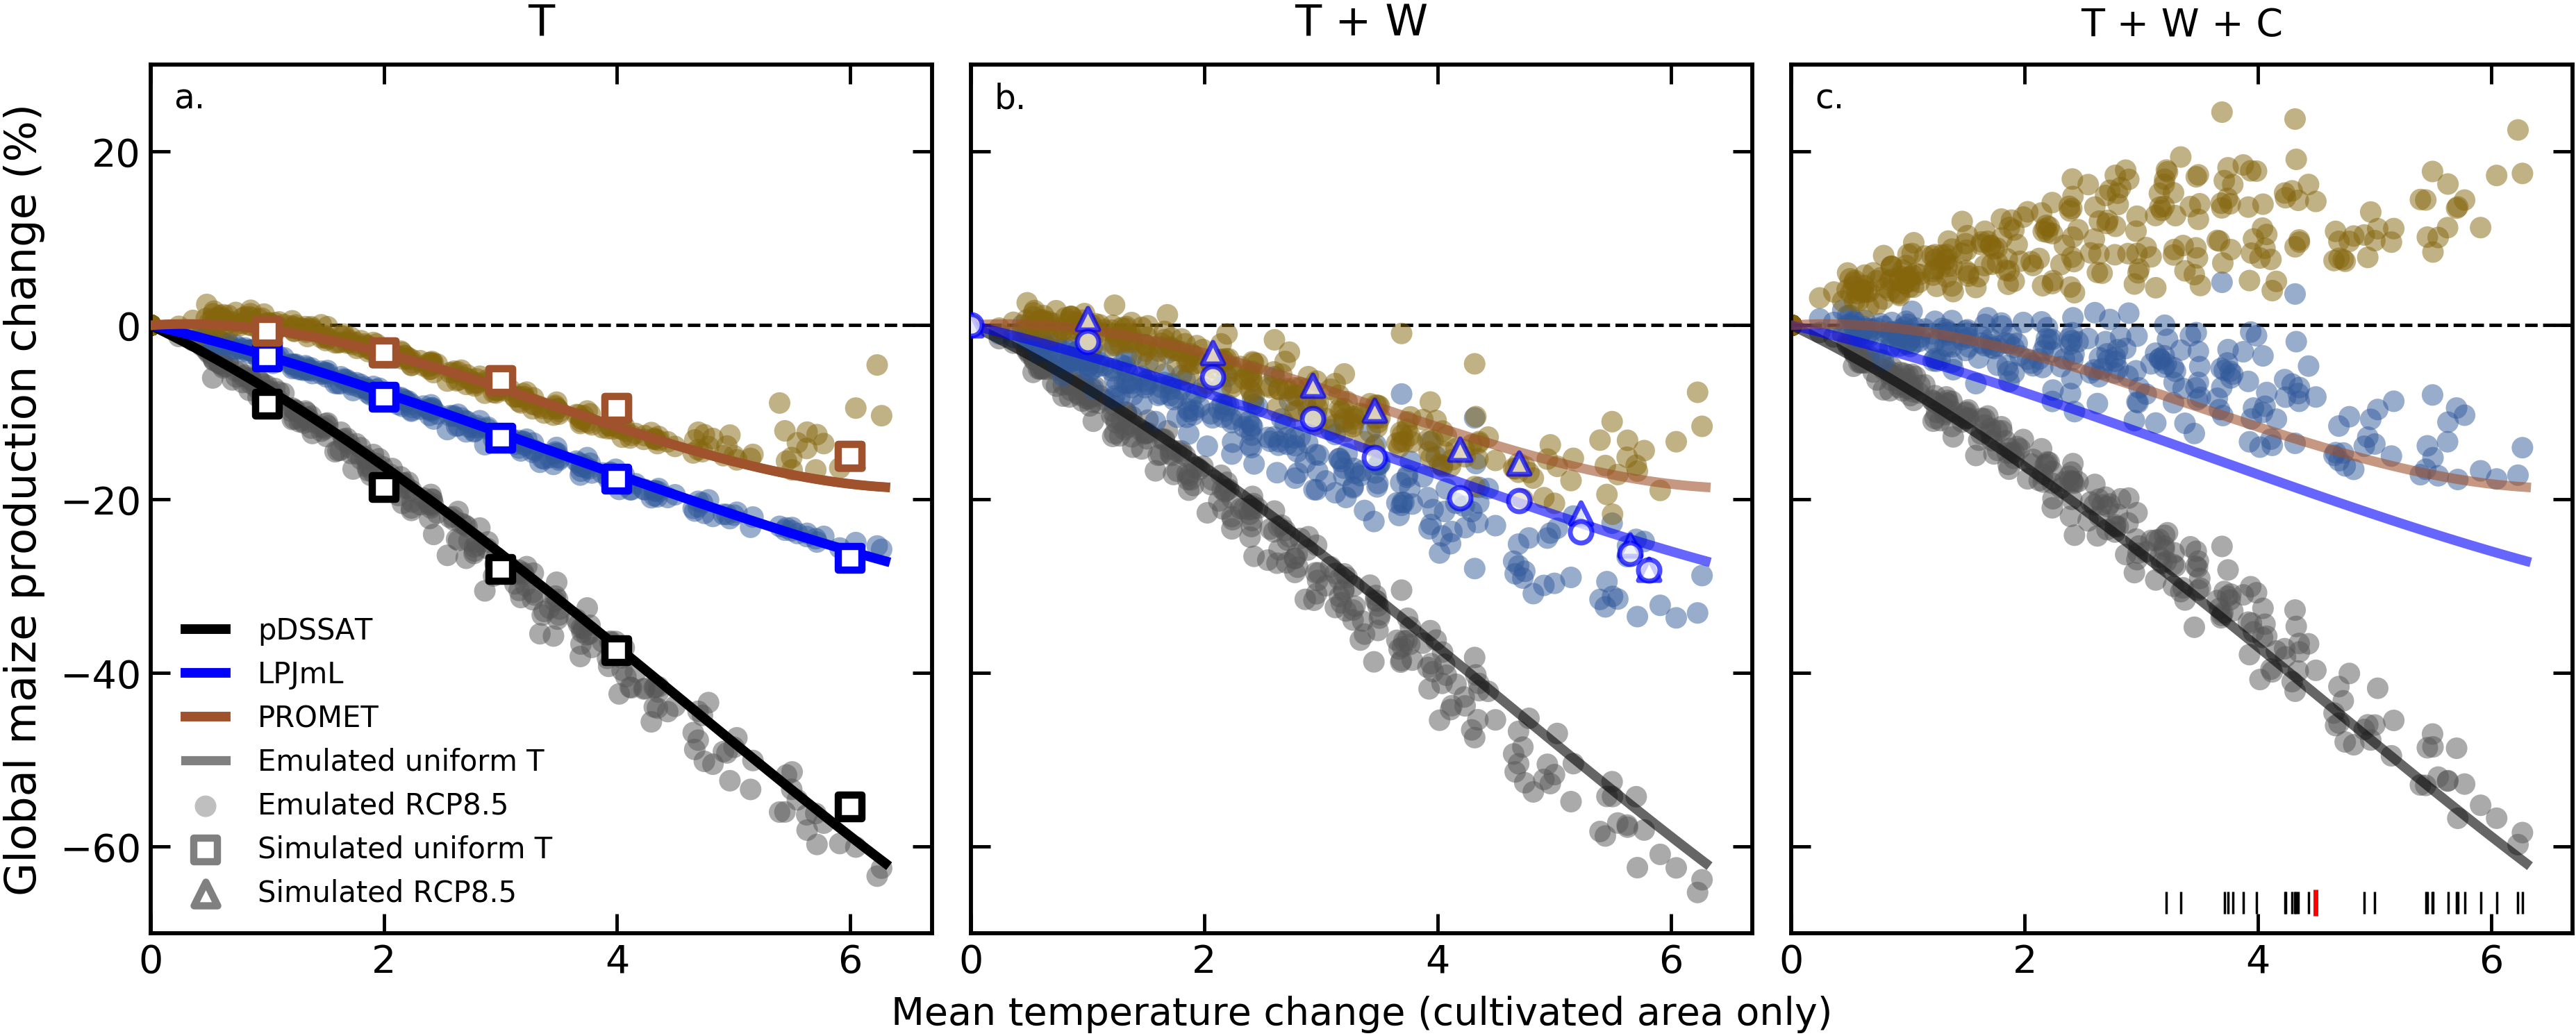
\includegraphics[width=8.3cm]{figures/global_em_maize.png}
    \caption{Global emulated damages for maize on currently cultivated lands for the GGCMI Phase II models emulated, for uniform temperature shifts with other inputs held at baseline. 
    (The damage function is created from aggregating up emulated values at the grid cell level, not from a regression of global mean yields.) 
    Lines are emulations for rainfed (solid) and irrigated (dashed) crops; for comparison, dots are the simulated values for the rainfed case.  
    For most models, irrigated crops show a sharper reduction than rainfed because of the locations of cultivated areas: irrigated crops tend to be grown in warmer areas where impacts are more severe for a given temperature shift (the exceptions are PROMET, JULES, and LPJmL). 
    For other crops and scenarios see Figures S18-21 in the supplemental material.}
    \label{fig:globe_em}
\end{figure}

\begin{figure*}[ht]
	\centering
    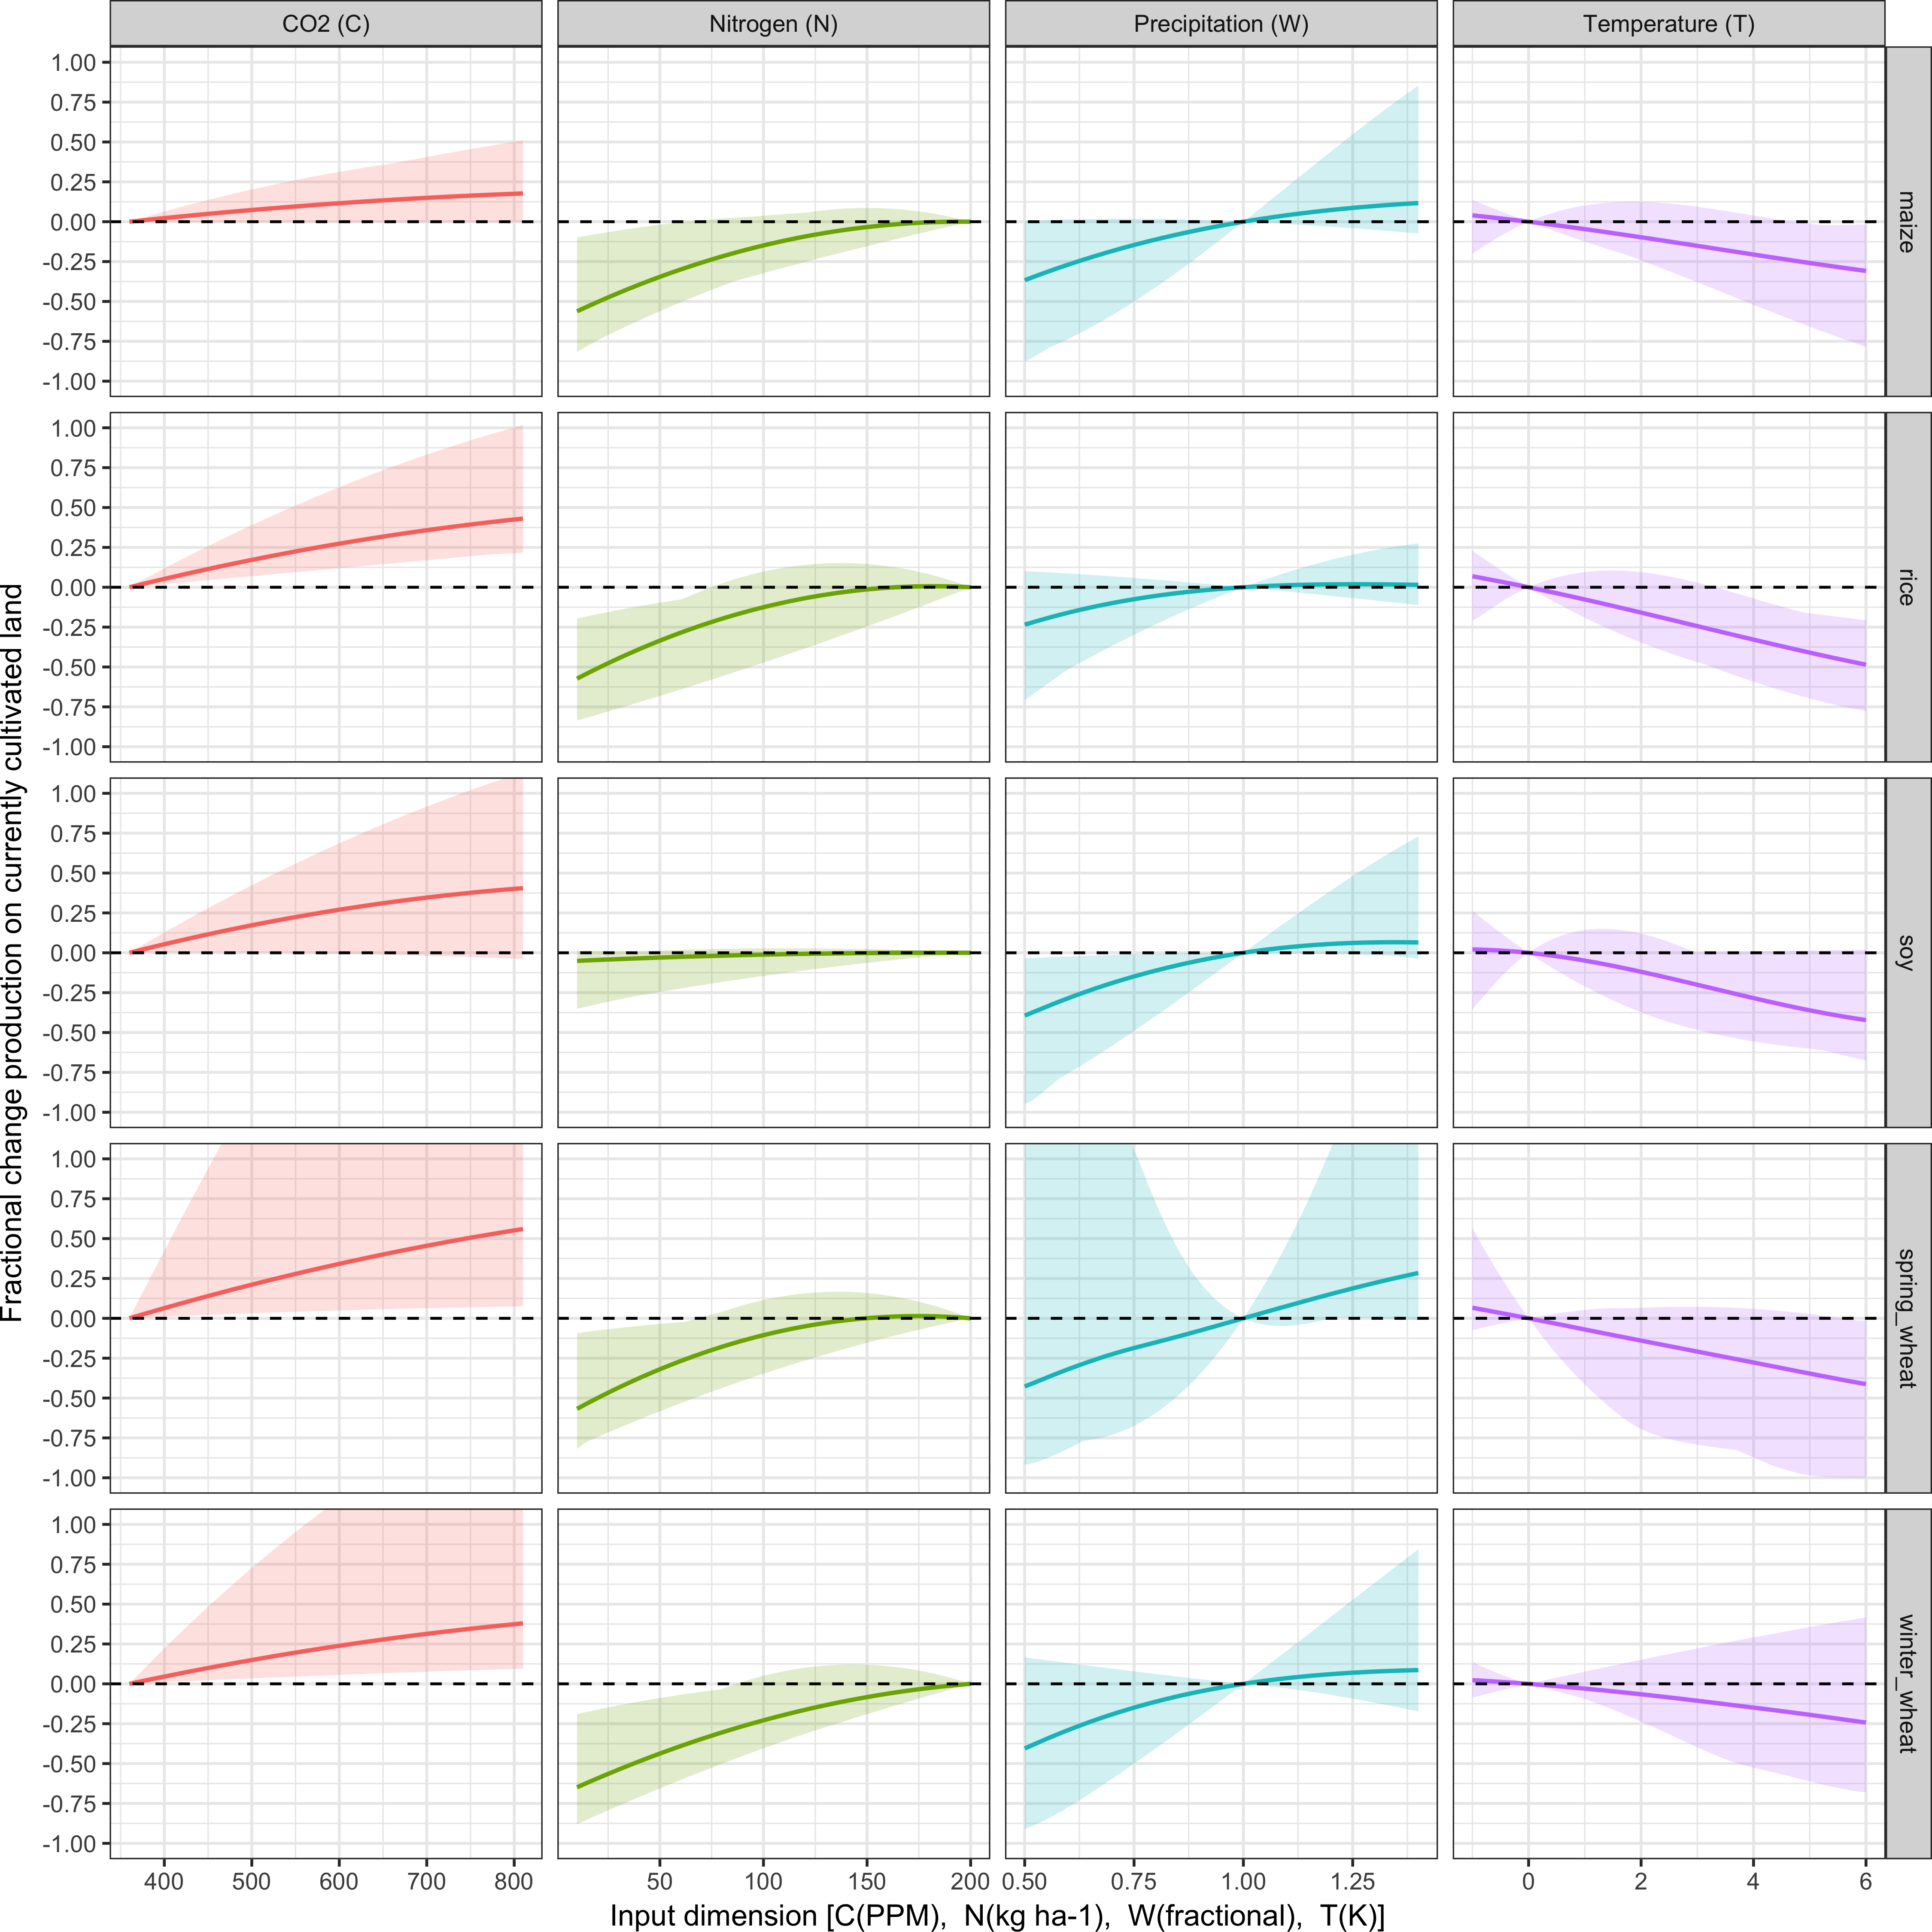
\includegraphics[width=15cm]{figures/em_CTWN_all_crops.png}
	\caption{Multi-model ensemble spread in sensitivity to changes in all four dimensions for crops at the global level. Minimum, MME mean and maximum model emulated damage function for currently cultivated areas. 
	PROMET and JULES removed from ensemble as they are the two models that are most difficult to emulate. 
	All other covariates held constant in each case and the fractional change in production is relative to the baseline case (T+0K, W+0\%, C=360ppm, and N=200kg ha-1).}
	\label{fig:all_dims}
\end{figure*}

Emulation provides not only a computational tool but a means of understanding and interpreting crop yield response across the parameter space. 
Emulation is only possible  when crop yield responses are sufficiently smooth and continuous to allow fitting with a relatively simple functional form, but this condition largely holds in the GGCMI Phase II simulations. 
Responses are quite diverse across locations, crops, and models, but in most cases local responses are regular enough to permit emulation. 
We show illustrations of emulation fidelity in this section; for more detailed discussion see Appendix B.

Crop yield responses are geographically diverse, even in high-yield and high-cultivation areas. 
Geographic diversity is high within a single crop and model (Figure \ref{fig:regression} rainfed maize in pDSSAT); this heterogeneity supports the choice of emulating at the grid cell level. 
Each panel in Figure \ref{fig:regression} shows simulated yield output from scenarios varying only along a single dimension (CO$_2$, temperature, precipitation, or nitrogen addition), with other inputs held fixed at baseline levels, compared to the full 4D emulation across the parameter space. 
Yields evolve smoothly across the space sampled, and the polynomial fit captures the climatological response to perturbations. 
Crop yield responses generally follow similar functional forms across models, though with a large spread in magnitude partly due to the lack of calibration. 
Inter-model diversity for a single crop and location is also high (Figure \ref{fig:regression_iowa}, rainfed maize in northern Iowa, also shown in Figure \ref{fig:regression}). 
Differences in response shape can lead to  differences in the fidelity of emulation, though comparison here is complicated by the different simulation experiment sampling regimes across models. 
Note that models are most similar in their responses to temperature perturbations. 

While the nitrogen dimension is important, it is also the most problematic to emulate in this work because of its limited sampling compared to other dimensions. 
The GGCMI Phase II protocol specified three nitrogen levels (10, 60 and 200 kg~N y$^{-1}$ ha$^{-1}$), so a third-order fit would be over-determined but a second-order fit can result in potentially unphysical results. 
Steep and nonlinear declines in yield with lower nitrogen levels mean that some regressions imply a peak in yield between the 100 and 200 kg~N y$^{-1}$ ha$^{-1}$ levels. 
While it is possible that over-application of nitrogen at the wrong time in the growing period could lead to reduced yields, these relative strength of this feature is are potentially an artifact of the fit. 
The Bayesian Ridge estimator tends to mitigate the `peak-decline effect' compared to ordinary least squares. 
In addition, the polynomial fit cannot capture the well-documented saturation effect of nitrogen application \citep[e.g.][]{Torsten77} as accurately as would be possible with a non-parametric model. 

The emulation fidelity demonstrated here is sufficient to allow using emulated response surfaces to compare model responses and derive insight about impacts projections. 
Because the emulator or ``surrogate model'' transforms the discrete simulation sample space into a continuous response surface at any geographic scale, it can be used for a variety of applications, including construction of continuous damage functions. 
As an example, we show a damage function constructed from the 4D emulation, aggregated to global yield, with simulated values shown for comparison (Figure \ref{fig:globe_em}, which shows maize on currently cultivated land; see Figures S18-S21 for other crops and dimensions). 
The emulated values closely match simulations even at this aggregation level. s
Soy as an efficient atmospheric nitrogen-fixer is relatively insensitive to nitrogen, and rice is not generally grown in water-limited conditions. Model spread is highest for spring wheat in general and for the CO$_2$ response for the wheats and soy.

Note that these functions are presented only as examples and do not represent true global projections, because they are developed from simulation data with a uniform temperature shift while increases in global mean temperature should manifest non-uniformly in space and distributions \citep{Sippel2015}. 
The global coverage of the GGCMI Phase II simulations allows impacts modelers to apply arbitrary geographically-varying climate projections, as well as arbitrary aggregation masks, to develop damage functions for any climate scenario and any geopolitical or geographic level bigger than 0.5 degrees in latitude and longitude.

\subsection{Emulator Assessment}
\label{S:4}
\begin{figure}[ht]
\centering
    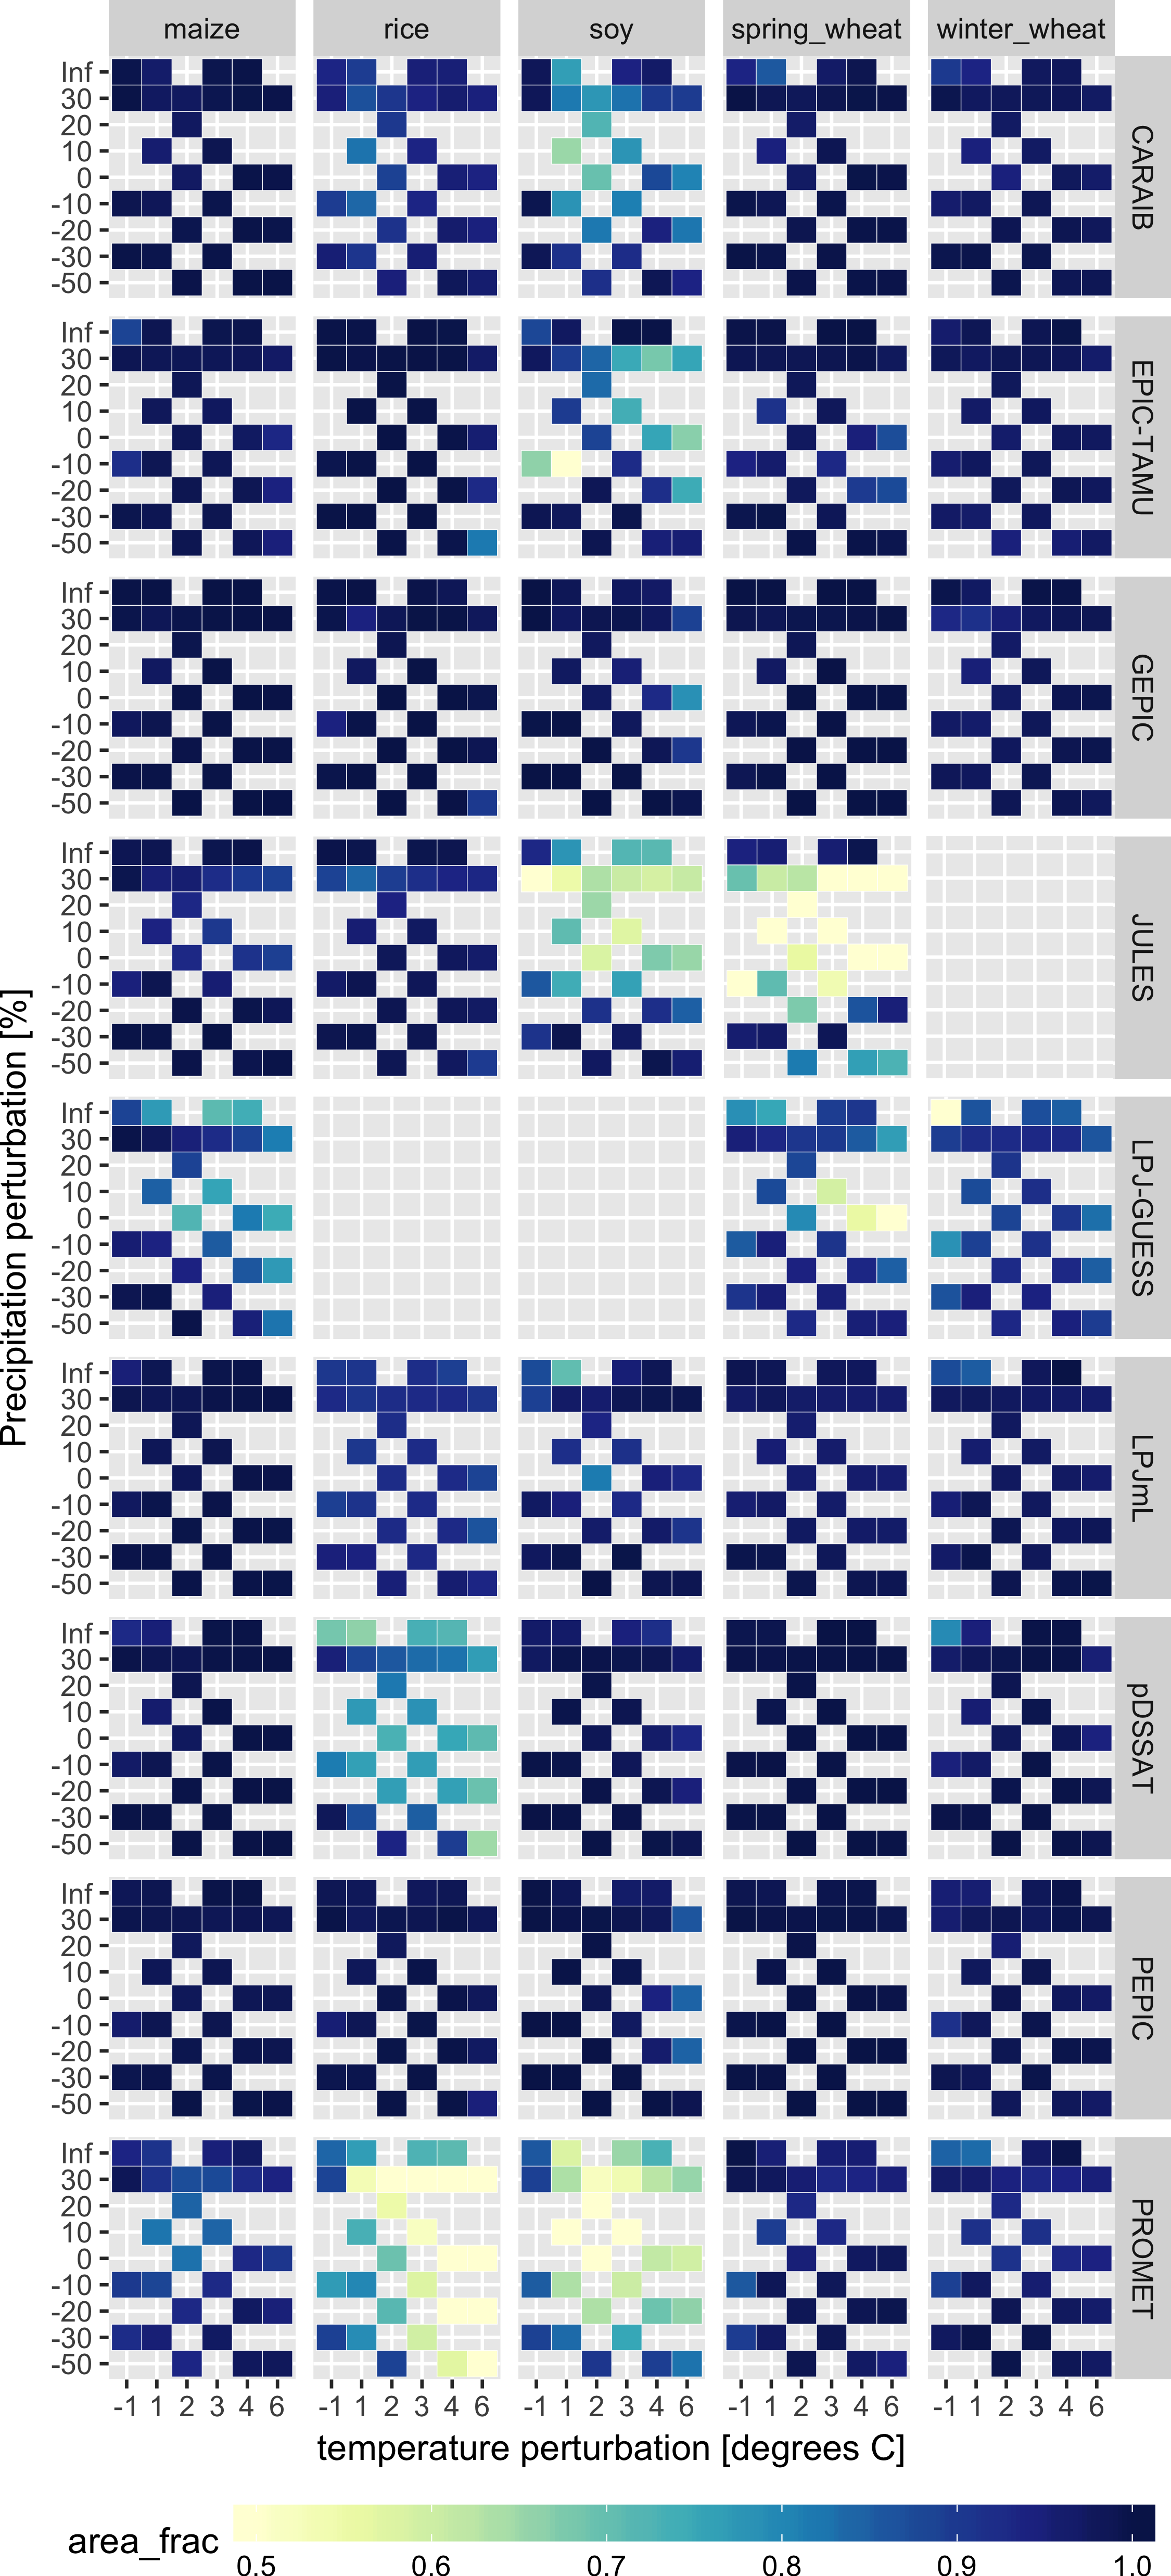
\includegraphics[width=6.5cm]{figures/error_360.png}
    \caption{Assessment of emulator performance over currently cultivated areas based on normalized error (Equations \ref{eqn:error}, \ref{eqn:per_yield}). 
    We show performance of all 9 models emulated, over all crops and all sampled T and P inputs, but with CO$_2$ and nitrogen held fixed at baseline values. 
    Large columns are crops and large rows models; squares within are T,P scenario pairs. 
    Colors denote the fraction of currently cultivated hectares ('area frac') for each crop with normalized area $e$ less that 1 indicating the the error between the emulation and simulation less that one standard deviation of the ensemble simulation spread. 
    Of the 756 scenarios with these CO$_2$ and N values, we consider only those for which all 9 models submitted data (Figure S3). 
    JULES did not simulate winter wheat and LPJ-GUESS did not simulate rice and soy. Emulator performance is generally satisfactory, with some exceptions. 
    Emulator failures (significant areas of poor performance) occur for individual crop-model combinations, with performance generally degrading for hotter and wetter scenarios.}
   \label{fig:error_360}
\end{figure}

\begin{figure}[ht]
\centering
    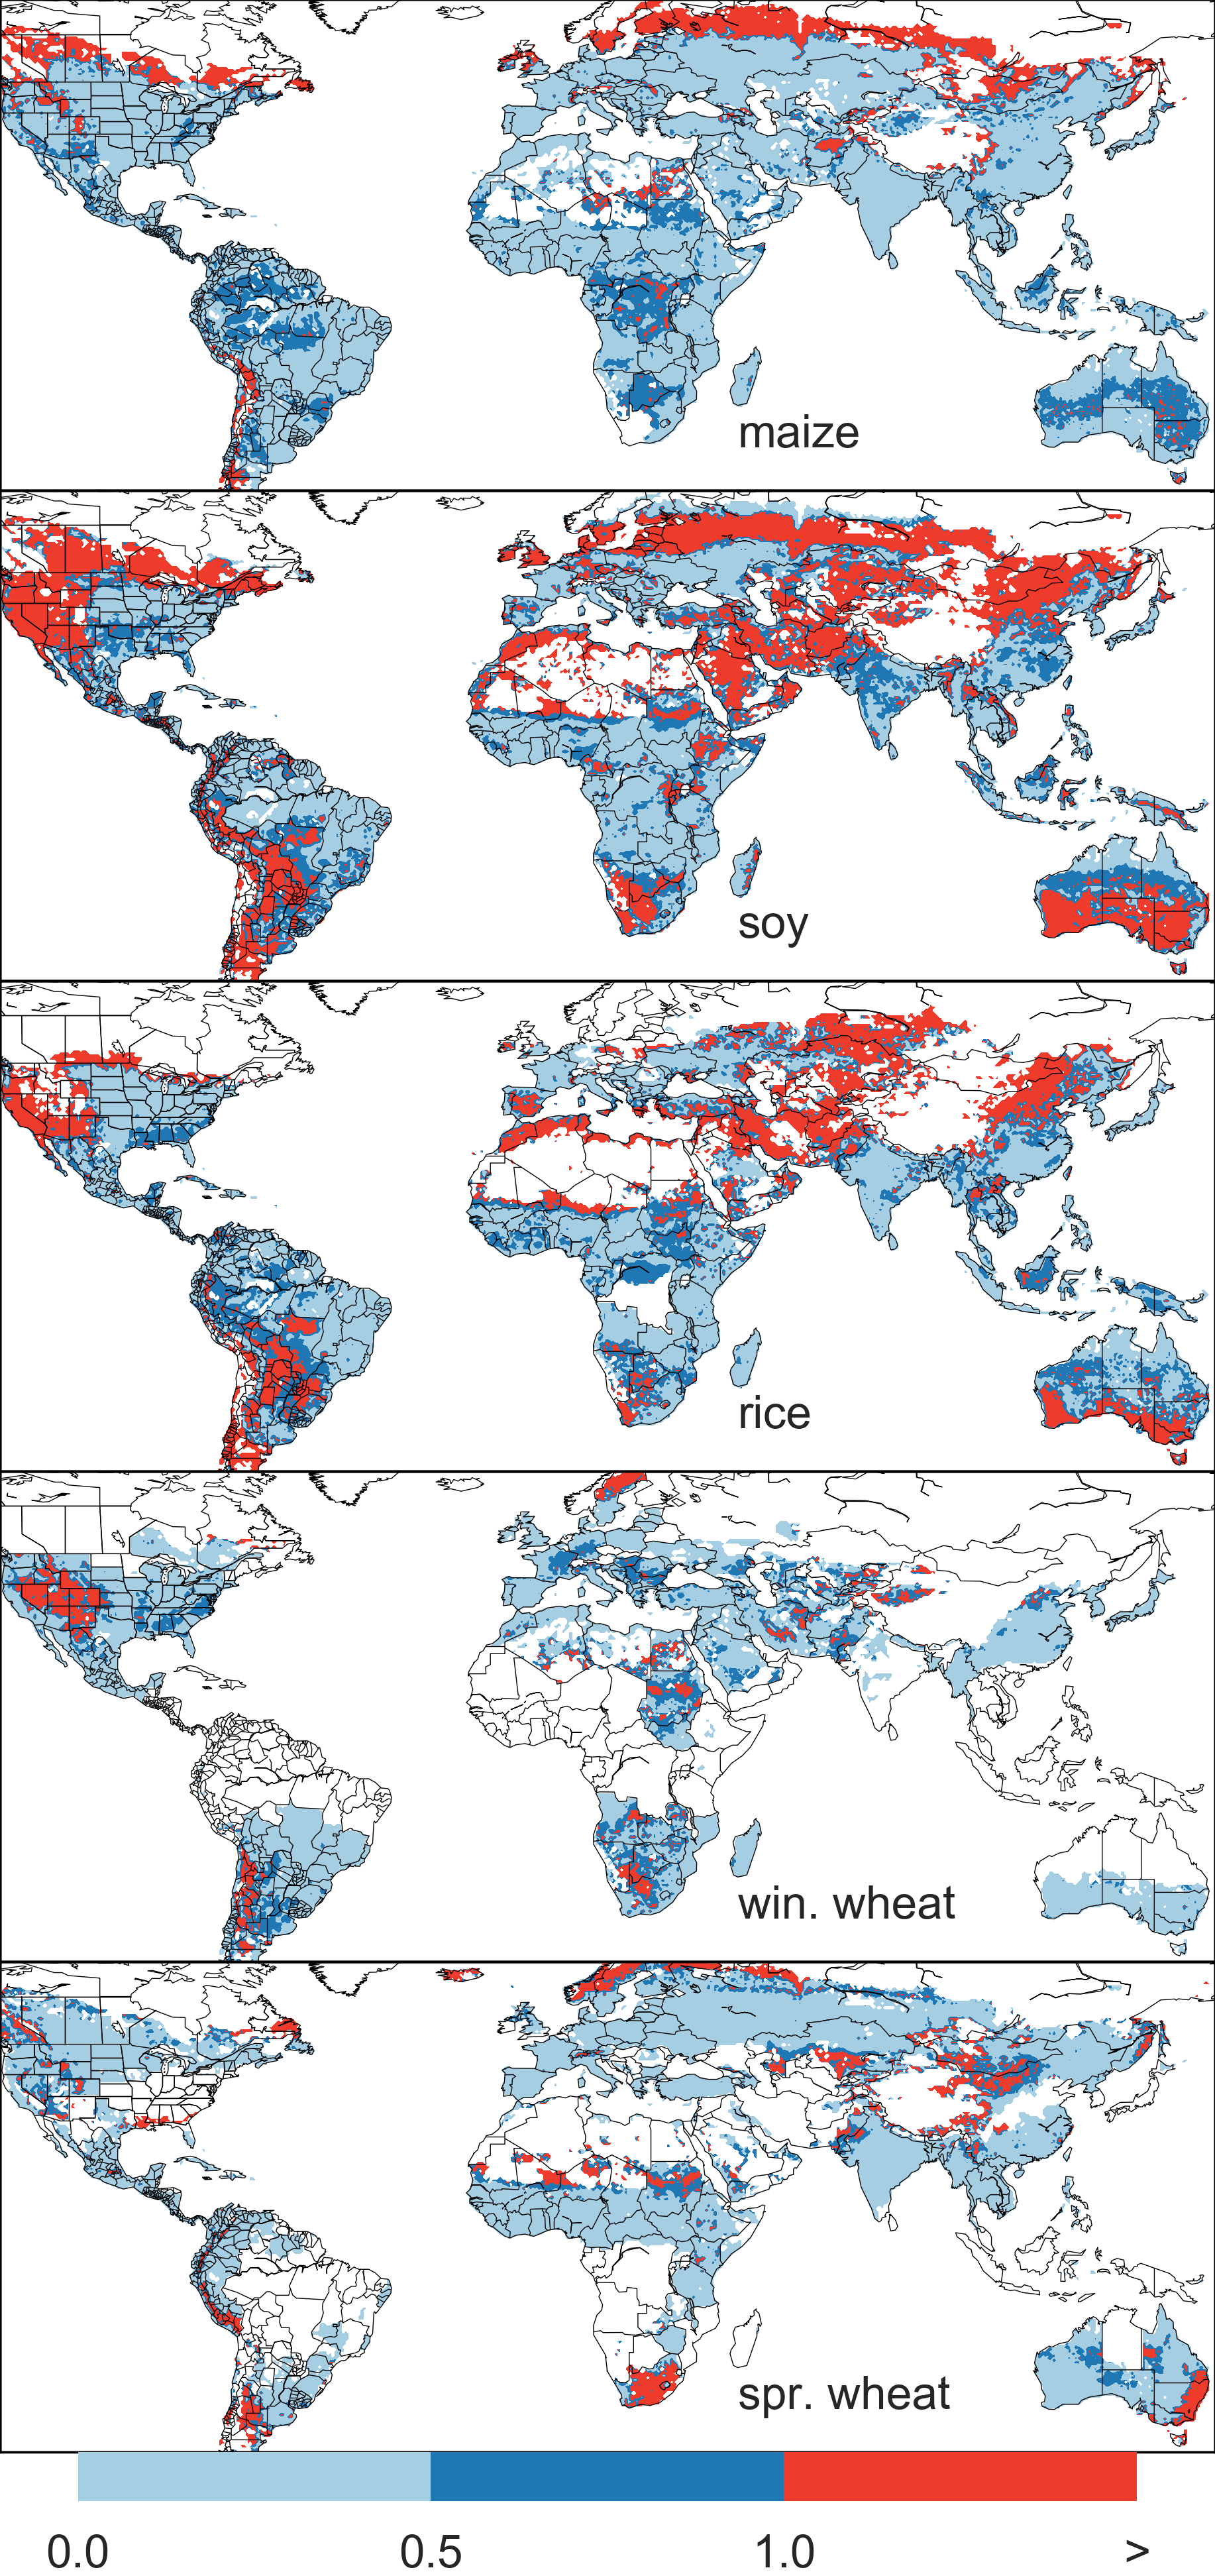
\includegraphics[width=6.5cm]{figures/em_err.png}
    \caption{Illustration of our test of emulator performance, applied to the CARAIB model for the T+4 scenario for rainfed crops. 
    Contour colors indicate the normalized emulator error $e$, where $e > 1$ means that emulator error exceeds the multi-model standard deviation. 
    White areas are those where crops are not simulated by this model. 
    Models differ in their areas omitted, meaning the number of samples used to calculate the multi-model standard deviation is not spatially consistent in all locations. 
    Emulator performance is generally good relative to model spread in areas where crops are currently cultivated (compare to Figure 1) and in temperate zones in general; emulation issues occur primarily in marginal areas with low yield potentials. 
    For CARAIB, emulation of soy is more problematic, as was also shown in Figure \ref{fig:error_360}.}
   \label{fig:error}
\end{figure}

\begin{figure*}[ht]
\centering
    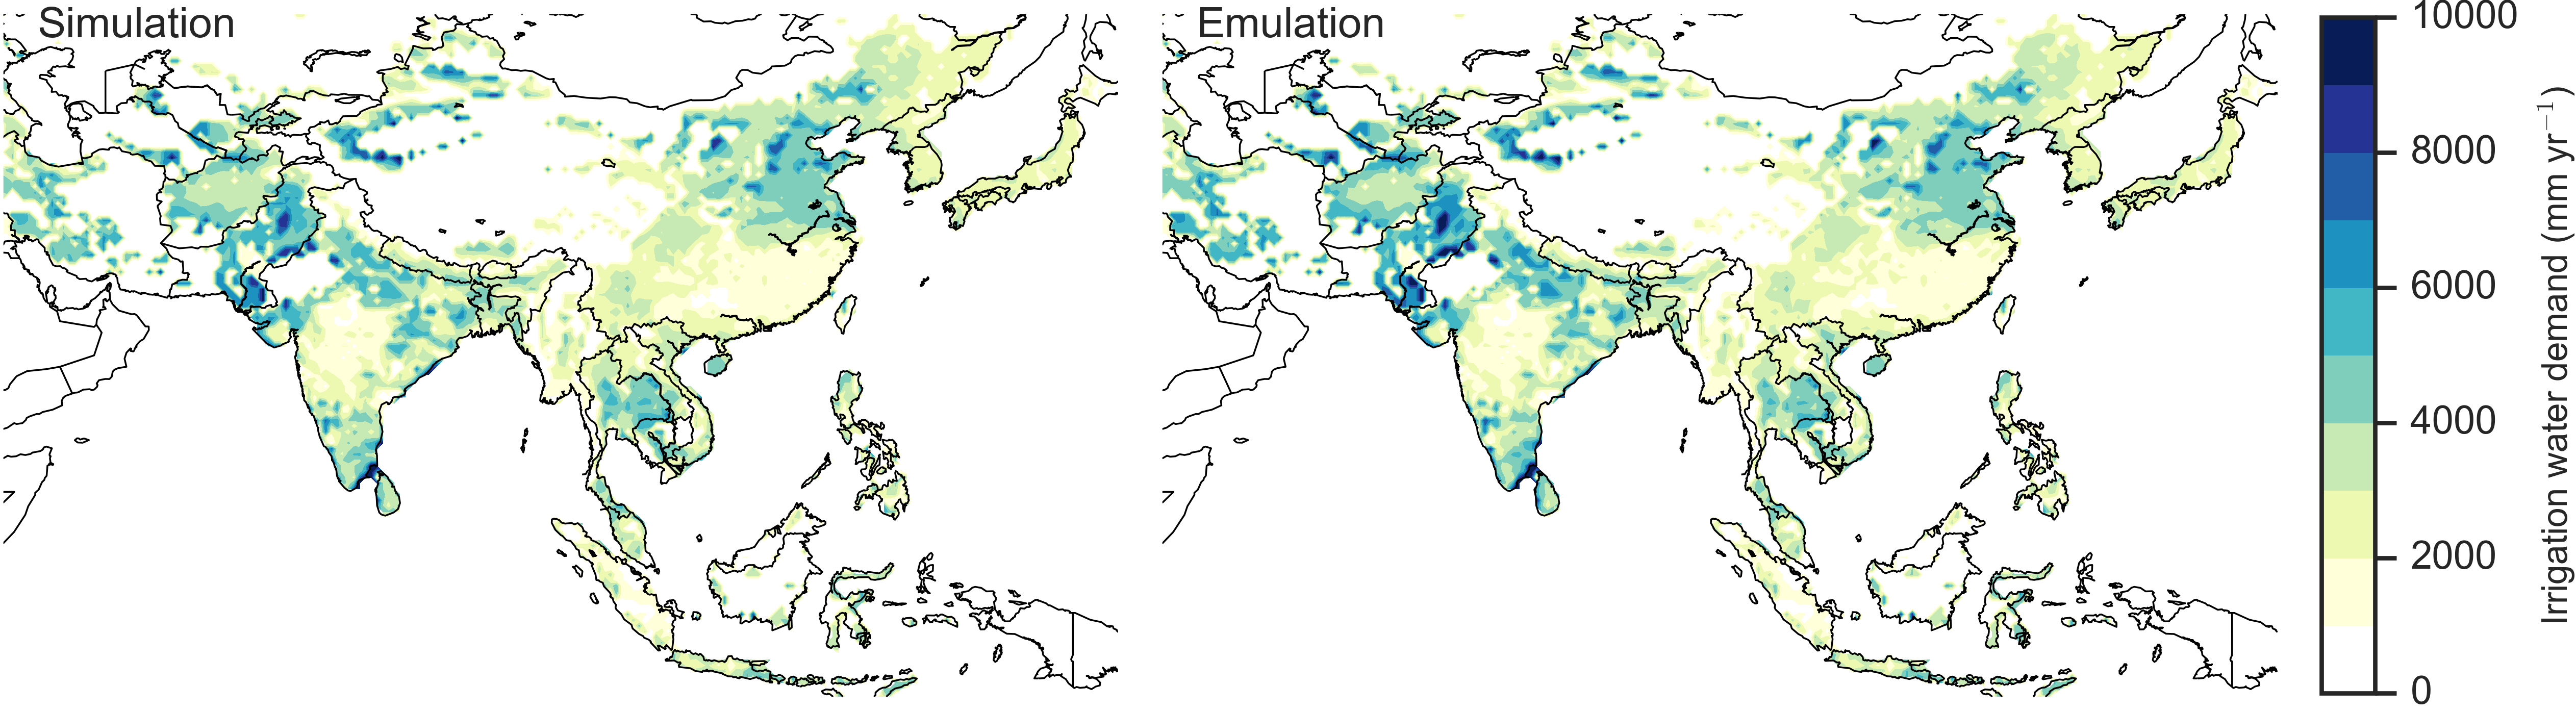
\includegraphics[width=16cm]{figures/irr_emulator_skill.png}
    \caption{Illustration of the spatial pattern of irrigation water demand.}
   \label{fig:error}
\end{figure*}

No general criteria exist for defining an acceptable crop model emulator, so we present two different metrics. 
First, for a multi-model comparison exercise like GGCMI Phase II, one reasonable criterion is what we term the ``normalized error'', which compares the fidelity of an emulator for a given model and scenario to the inter-model uncertainty. 
We define the normalized error $e$ for each scenario as the difference between the fractional yield change from the emulator and that in the original simulation, divided by the standard deviation of the multi-model spread (Equations \ref{eqn:per_yield} and  \ref{eqn:error}):

\begin{equation}
    \label{eqn:per_yield}
    F_{\: scn.}=\frac{Y_{scn.}-Y_{baseline}}{Y_{baseline}}
\end{equation}

\begin{equation}
    \label{eqn:error}
    e_{\: scn.} =\frac{F_{em, \: scn.}-F_{sim, \: scn.}}{\sigma_{sim, \: scn.}}
\end{equation}

Here $F_{\: scn.}$ is the fractional change in a model's mean emulated or simulated yield from the defined historical baseline, in a certain setting or scenario (scn.) in C, T, W, and N space; $Y_{scn.}$ and $Y_{baseline}$ are the absolute emulated or simulated mean yields. 
The normalized error $e$ is the difference between the emulated fractional change in yield and that actually simulated, normalized by $\sigma_{sim}$, the standard deviation in simulated fractional yields change $F_{sim,\: scn.}$ across all models. 
The emulator is fitted across all available simulation outputs for each grid cell, model, and crop, and then the error is calculated across the each of the simulation scenarios provided by all nine models (Figure S3). 

This metric implies that emulation is generally satisfactory, with several distinct exceptions. 
Almost all model-crop combination emulators have normalized errors less than one over nearly all currently cultivated hectares (Figure \ref{fig:error}), but some individual model-crop combinations are difficult to emulate (e.g.\ PROMET for rice and soy, JULES for soy and spring wheat, Figures S24-S25). 
Problems with emulating PROMET for rice and soy may have to do with the parametrization of the phenology for those crops which lengthens the growing season in some cases. 
Normalized errors for soy are somewhat higher across all models not because emulator fidelity is worse but because models agree more closely on yield changes for soy than for other crops (see Figure S18), lowering the denominator. 
Emulator performance often degrades in geographic locations where crops are not currently cultivated. 
For example, emulator performance may be satisfactory over cultivated areas for all crops, but uncultivated regions may show some problematic areas (Figure \ref{fig:error} shows a CARAIB model case, see also Figure S26).

This first assessment procedure is relatively forgiving for several reasons. 
First, each emulation is evaluated against the simulation actually used to train the  (in-sample validation). 
Had we used a spline interpolation the error would necessarily be zero. 
Second, the performance metric scales emulator fidelity not by the magnitude of yield changes but by the inter-model spread in those changes. 
The normalized error $e$ for a model depends not only on the fidelity of its emulator in reproducing a given simulation but on the particular suite of models considered in the intercomparison exercise. 
Where models differ more widely, the standard for emulators becomes less stringent. 
This effect is readily seen when comparing assessments of emulator performance in simulations at baseline CO$_2$ (Figure \ref{fig:error_360}) with those at higher CO$_2$ levels (Figure S27) because models disagree on the magnitude of CO$_2$ fertilization. 
The rationale for this choice of assessment metric is to relate the fidelity of the emulation to an estimate of true uncertainty, which we take as the multi-model spread. 
We therefore do not provide a formal parameter uncertainty analysis, but note that the GGCMI Phase II dataset is well-suited to statistical exploration of emulation approaches and quantification of emulator fidelity. 
More rigorous emulator assessments that could be preformed in future work include: testing other statistical specifications including non-parametric models and calculating standard error on emulator parameters.

We also provide a more stringent test of emulator performance; a three-fold cross validation (out-of-sample validation). 
Here the training data is split and the model is trained on two thirds of the data and tested on the held out portion (the process is then repeated three times to cover all data in the training set). 
We normalize the error in each grid cell by dividing by the yield in that grid cell in the baseline (T+0, W+0, C=360, N=200) case and show aggregations by grid cell and weighted by area cultivated per grid cell. 
Errors are generally low as a percentage of yield --even for this strict protocol-- and when weighted by area, essentially zero in most cases (Table \ref{table:ASE}). 
Note that the cross validation process often does not include edge simulations in the training set that are then predicted in the test phase. 
This extrapolation during cross validation is not representative based on the intended use of the emulator.

\begin{table*}[t]
\caption{Mean absolute error of emulator representation of a simulation as a percentage of baseline yield for the cross-validation process. 
A 3-fold stratified k-fold cross validation scheme is utilized where the model is trained on two-thirds of the data and validated on the held-out remaining third (repeated three times). 
The split does not represent a uniform number of samples in each location or in each model because simulation sampling extent in variable spaces is heterogeneous. 
The calculation only includes grid cells with at least 1 \% of surface area cultivated with a specific crop (approximately 1000 grid cells in each case). 
The table displays area weighted mean (`WM') shows the mean error weighted by hectares grown in each grid cell \citep{Portmann2010} and `MD' shows the unweighted median across grid cell values. 
* Indicates cases where the OLS linear model is unstable.} 
\label{table:ASE}
\begin{tabular}{l | cc | cc | cc | cc | cc} 
\hline
{} & \multicolumn{2}{c|}{\textbf{Maize}} & \multicolumn{2}{c|}{\textbf{Soy}}& \multicolumn{2}{c |}{\textbf{Rice}} & \multicolumn{2}{c |}{\textbf{S. Wheat}} & \multicolumn{2}{c}{\textbf{W. Wheat}} \\
\textbf{Model}     & WM (\%)& MD (\%)& WM (\%)& MD (\%)& WM (\%)& MD (\%)& WM (\%)& MD (\%)& WM (\%) & MD (\%) \\ \hline
\textbf{CARAIB}    & 0.00  & 1.71  & 0.02  & 2.39  & 0.03  & 2.95  & 0.02  & 4.40  & 0.01  & 2.36  \\ \hline
\textbf{EPIC-TAMU} & 0.00  & 4.30  & 0.01  & 6.24  & 0.00  & 3.35  & 0.01* & 6.82* & 0.01  & 3.51  \\ \hline
\textbf{JULES}     & 0.11  & 6.13  & 0.01  & 10.2  & 0.01  & 6.97  & 0.04  & 15.1  & NA    & NA    \\ \hline
\textbf{GEPIC}     & 0.00  & 5.78  & 0.00  & 3.75  & 0.01  & 5.64  & 0.01  & 6.76  & 0.01  & 7.01  \\ \hline
\textbf{LPJ-GUESS} & 0.00  & 1.78  & NA    & NA    & NA    & NA    & 0.05  & 6.22  & 0.02  & 3.35  \\ \hline
\textbf{LPJmL}     & 0.00  & 9.44  & 0.00  & 3.25  & 0.01  & 8.37  & 0.01  & 9.83  & 0.01  & 4.98  \\ \hline
\textbf{pDSSAT}    & 0.00  & 2.93  & 0.05  & 3.02  & 0.01  & 3.97  & 0.01  & 2.97  & 0.01  & 4.67  \\ \hline
\textbf{PROMET}    & 0.01  & 4.19  & 0.00  & 6.03  & 0.01  & 9.85  & 0.01  & 7.04  & 0.01  & 3.68   \\ \hline
\textbf{PEPIC}     & 0.00* & 3.71* & 0.00* & 2.80* & 0.00* & 2.89* & 0.00* & 4.83* & 0.02* & 6.70*  \\ \hline
\end{tabular}
\end{table*}

%%%%%%%%%%%%%%%%%%%%%%%%%%%%%%%%%%%%%%%%%%%%%%%%%%%%%%%%%%%%%%%
%%%%%%%%%%%%%%%%%%%%%%%%%%%%%%%%%%%%%%%%%%%%%%%%%%%%%%%%%%%%%%%
%%%%%%%%%%%%%%%%%%%%%%%%%%%%%%%%%%%%%%%%%%%%%%%%%%%%%%%%%%%%%%%

\section{Discussion and Conclusions} 
\label{S:5}
We show that the systematic parameter sampling in the GGCMI Phase II experiments allow emulating climatological crop yield responses with a relatively simple reduced-form statistical model. 
The sampling provides information on the influence of multiple interacting factors in a way that realistic climate model simulations cannot, and allows isolating long-term impacts from confounding factors that lead to different year-over-year responses. 
The use of a relatively simple functional form in turn offers the possibility of physical interpretation of parameter values that can assist in model intercomparison and evaluation. 

...several cautions need to be noted. While the emulator allows estimating agricultural impacts under arbitrary climate scenarios, extrapolation outside the sample space should be avoided. 
Additionally, because the simulation protocol was designed to focus on change in yield under climate perturbations and not on replicating real-world yields, the models are not formally calibrated so cannot be used for impacts projections except in conjunction with historical yield information. 
Finally, because the GGCMI Phase II simulations apply uniform perturbations to historical climate inputs, they do not sample potential changes in climate variability. 
Although such changes are uncertain and remain poorly characterized \citep[e.g.][]{Alexande2006, Kodra2014}, follow-up experiments may wish to consider them. 
Several recent studies have described procedures for generating simulations that combine historical data with model projections of changes in the marginal distributions or temporal dependence of temperature and precipitation(e.g.\ \citet{Leeds2015, poppick2016, Won16} and \citet{Haugen2018}).

The GGCMI Phase II dataset invites a broad range of potential future avenues of analysis, especially because emulation allows statistical distillation of the large dataset (40 billion simulated yields) into a tractable form. 
Potential studies might include a detailed examination of interaction terms between the major input drivers, robust quantification of model sensitivities to input drivers, exploration of yield responses to extremes, and evaluation of geographic shifts in optimal growing regions. 
The dataset also enables studies of emulation itself, including a more systematic evaluation of different statistical model specifications and formal calculation of uncertainties in derived parameters. 
In general, the development of multi-model ensembles involving systematic parameters sweeps has large promise for better understanding potential future crop responses and for improving process-based crop models.

%%%%%%%%%%%%%%%%%%%%%%%%%%%%%%%%%%%%%%%%%%%%%%%%%%%%%%%%%%%%%%%
\codedataavailability{The polynomial emulator parameter matrices for all crop model emulators are available at {doi.org/10.5281/zenodo.2605374.}}

%\appendix
%\section{}
%\subsection{Data Access}
%\noappendix %% use this to mark the end of the appendix section

\authorcontribution{J.E., C.M, A.R., J.F., and E.M.\ designed the research. C.M., J.J., J.B., P.C., M.D., P.F., C.F., L.F., M.H., C.I., I.J., C.J., N.K., M.K., W.L., S.O., M.P., T.P., A.R., X.W., K.W., and F.Z.\ performed the simulations. J.F., J.J., A.S., M.L., and E.M.\ performed the analysis and J.F. and E.M.\ prepared the manuscript.}

\competinginterests{The authors declare no competing interests.}

\begin{acknowledgements}
We thank Michael Stein and Kevin Schwarzwald, who provided helpful suggestions that contributed to this work. 
This research was performed as part of the Center for Robust Decision-Making on Climate and Energy Policy (RDCEP) at the University of Chicago, and was supported through a variety of sources. 
RDCEP is funded by NSF grant \#SES-1463644 through the Decision Making Under Uncertainty program. J.F.\ was supported by the NSF NRT program, grant \#DGE-1735359. 
C.M.\ was supported by the MACMIT project (01LN1317A) funded through the German Federal Ministry of Education and Research (BMBF). 
C.F.\ was supported by the European Research Council Synergy grant \#ERC-2013-SynG-610028 Imbalance-P. 
P.F.\ and K.W.\ were supported  by the Newton Fund through the Met Office Climate Science for Service Partnership Brazil (CSSP Brazil). 
K.W.\ was supported by the IMPREX research project supported by the European Commission under the Horizon 2020 Framework programme, grant \#641811. 
A.S.\ was supported by the Office of Science of the U.S. Department of Energy as part of the Multi-sector Dynamics Research Program Area. 
S.O.\ acknowledges support from the Swedish strong research areas BECC and MERGE together with support from LUCCI (Lund University Centre for studies of Carbon Cycle and Climate Interactions). 
R.C.I.\ acknowledges support from the Texas Agrilife Research and Extension, Texas A \& M University. 
This is paper number 35 of the Birmingham Institute of Forest Research. 
Computing resources were provided by the University of Chicago Research Computing Center (RCC).
\end{acknowledgements}

%% Since the Copernicus LaTeX package includes the BibTeX style file copernicus.bst,
\bibliographystyle{copernicus}
\bibliography{bib}

\end{document}